

% !TeX spellcheck = en_US
\documentclass[12pt]{article}
\usepackage{graphicx} % Required for inserting images
\usepackage{float}
\usepackage{hyperref}
\usepackage[utf8]{inputenc}
\usepackage[english]{babel}
\usepackage[backend=bibtex,style=trad-plain,bibencoding=utf8]{biblatex}
\usepackage{pythonhighlight}



\usepackage{csquotes}
\usepackage{comment}

\graphicspath{ {./img/} }
\addbibresource{llm.bib}

\title{Titolo}
\author{Pietro Bertorelle}

\date{June 2025}

\begin{document}


\begin{titlepage}
    \begin{center}

        
\includegraphics[width=0.60\textwidth]{Logo_PoliTo_dal_2021_blu.png}

        \vspace*{0.5cm}

        \LARGE
        \textbf{Politecnico di Torino}

        \vspace{0.5cm}
        \LARGE
        Computer Engineering

        \vspace*{1cm}
            
        \Huge
        \textbf{Stress testing chatbots: evaluating factuality, reasoning, abstraction, and other safety challenges}
            
                    
        \vspace{1.5cm}

        \Large
        \begin{minipage}[t]{0.4\textwidth}
             \textbf{Candidate:}
        \end{minipage}
        \hfill
        \begin{minipage}[t]{0.45\textwidth}
            \raggedleft
            Pietro Bertorelle
        \end{minipage}
            
            
        \vspace{1cm}
            
           
        \Large
        \begin{minipage}[t]{0.4\textwidth}
             \textbf{Supervisors:}
        \end{minipage}
        \hfill
        \begin{minipage}[t]{0.45\textwidth}
            \raggedleft
            Antonio Vetr\'o\\
            Marco Rondina\\
        \end{minipage}
        
        \vspace{2cm}
        Academic Year 2024/25
            
    \end{center}
\end{titlepage}




\clearpage
\begin{abstract}
The widespread use of Large Language Models (LLMs) in complex tasks has highlighted significant risks, including misinformation and biases. Moreover, the introduction of ``agentic AI'' concept---autonomous systems capable of performing tasks without human intervention---encourages the use of LLMs for tasks they are not designed for. In response, agentic benchmarks were introduced to assess the reliability of these models on real-world tasks.

This thesis proposes a benchmark with the aim of understanding the state-of-the-art in complex planning, factual accuracy and mathematical problem-solving, by analyzing the most popular chatbots from a technical point of view and the risks they entail.

The benchmark tests were performed on Gemini, Gemma, and Llama, spanning 10 different versions of these models. This benchmark consists of 22 questions repeated more than 273,000 times using different prompting methodologies, such as zero-shot Chain of Thought (CoT), in which the model is asked to solve the problem step-by-step, and Program of Thought (PoT), which requires writing Python code that solves the problem.

The benchmark results identify several limitations in the tasks analyzed and the direction of development of some models. Specifically, the resolution of mathematical tasks with Gemini has improved significantly with the progress of versions and, in general, all analyzed models were more accurate in this category than in planning. Some limitations in the use of the PoT methodology can also be identified in real-world mathematical problems, where the use of 0-shot CoT improves accuracy.\\ 
Testing the factuality category revealed that LLMs struggle to recognize an incorrect statement or a trick question. Meanwhile, analysis of planning ability revealed an incapability to handle overlapping plans in the submitted questions. For instance, all LLMs achieved results close to 0\% accuracy when the problems involved performing seemingly contradictory sub-actions to achieve the result, as in ``Tower of Hanoi'' or ``Blocks World''.

The findings highlight some of LLMs' current challenges to achieve agency, such as their inability to handle complex planning and factual nuances. Even in the mathematical domain, where the best results were achieved, the necessity of a third-party intervention has been shown.

Tests like those conducted in this study will better identify the robustness of new agents, and also point to the need for greater granularity in existing benchmarks of LLMs' capabilities to ensure their responsible use.


\end{abstract}

\clearpage

\textbf{Acknowledgments}

I would like to thank my parents for all their support during my years of study, my family and my friends for being there for me when I needed them, and my comrades for everything we have achieved together.
\clearpage
\tableofcontents
\clearpage
\listoffigures
\clearpage

\section{Introduction}

Large Language Models (LLMs) are stochastic systems that produce outputs by drawing relevant content from their datasets, based on patterns they've autonomously identified during training. By their very nature, these probabilistic tools shouldn't have widespread applicability. However, thanks to marketing campaigns over the last few years, they've been introduced as multi-purpose tools aimed at replacing humans in a wide range of tasks.\\
Indeed, free mass access and their excellent performance in certain tasks make them appealing, but the new concept of \textbf{Agentic AI}, adopted by most producing companies, goes further, hypothesizing their use in any task without human supervision.\\
The challenge lies in measuring their true reliability. Currently, this is relegated to benchmarks, which are often incomprehensible to the end-user and are used as a metric for improvement by a niche of industry professionals.

This thesis proposes an \textbf{agentic benchmark} that, while limited, can clearly identify the strengths and weaknesses of current models by creating novel problems across three main categories: \textbf{reasoning}, \textbf{factuality}, and \textbf{sequential problem solving}. This last category is designed to test planning abilities on problems of discrete complexity.\\ 
Given the generality of these three categories, the questions are grouped into sub-categories by problem type for greater data clarity, as shown in Figure \ref{fig:finalBench}.\\
The thesis is divided into three chapters:
\begin{itemize}
\item \textbf{Background}: Analyzes the foundational technologies of LLMs, the concept of agentic benchmarks, and the results available in the technical reports of recent models on various benchmarks.
\item \textbf{Methodology}: Explains how the question categories were identified, the prompting methodologies used, and how the experiment was set up.
\item \textbf{Results}: Presents the findings obtained during the testing phase.
\end{itemize}

The models tested include the Gemini 1.5 and 2.0 families, Gemma 3 with 1B and 4B parameters, and Llama 3.1 8B and Llama 3.2 1B and 3B.\\
The findings reveal a clear performance hierarchy. On classic math problems, Gemini models achieve an accuracy close to $100\%$ using the PoT (Program-of-Thought) methodology. The larger parameter versions of Gemma and Llama also get approximately $50\%$ of accuracy in the same category. \\
As the math problems increase in complexity, Gemini's latest versions maintain decent results, while the 1.5 family's performance degrades and the open models struggle, with scores dropping to nearly $0\%$.\\
Sudoku solving was only tested on Gemini models, and all provided solutions were incorrect.\\
In factuality category, when presented with logical trick questions, all models had an accuracy close to $0\%$.\\
In sequential problem solving, open models consistently gave incorrect answers. Gemini models also had $0\%$ accuracy, except for Gemini 2.0 Flash, which achieved an average of about $10\%$.

\clearpage
\section{Background}
    \subsection{Large Language Models (LLMs)}
A Large Language Model (LLM) is a computational model, based on \textbf{neural networks}, trained on a vast amount of data, with the purpose of processing natural languages.\\
The most capable LLMs are \textbf{generative pretrained transformers (GPTs)}, which are largely used in generative chatbots such as \textbf{ChatGPT} and \textbf{Gemini}. GPT consists of an artificial neural network, pre-trained on large datasets of unlabeled text and based on the \textbf{transformer architecture}.

    \subsubsection{Neural Networks (NNs)}
A neural network is a model that consists of different layers of nodes connected to one another.\begin{figure}[H]
\centering
        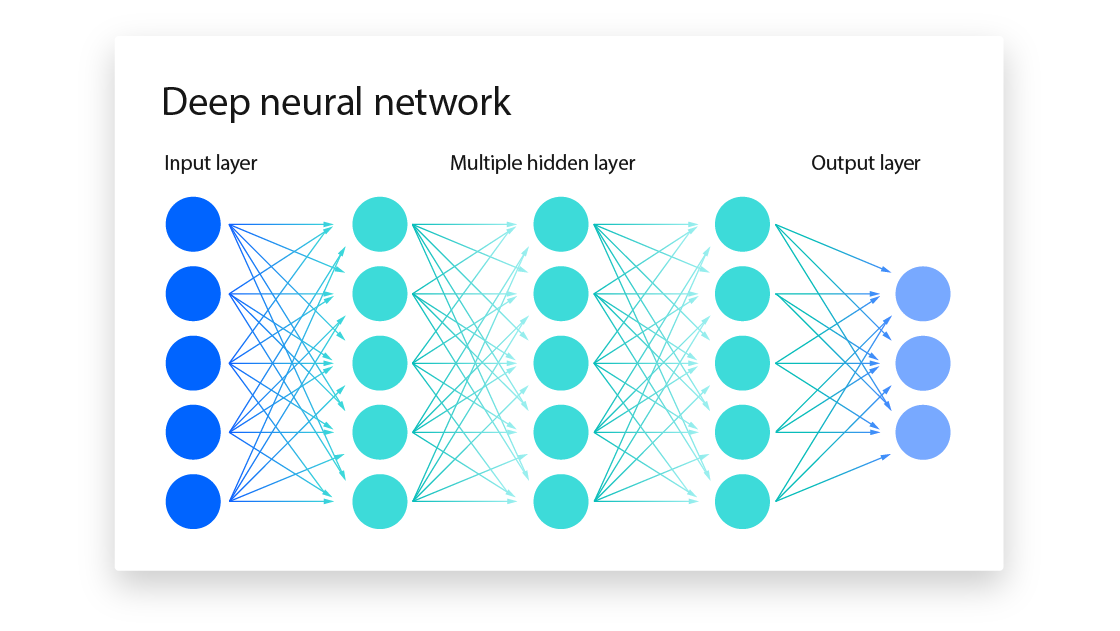
\includegraphics[width=1\textwidth]{DeepNeuralNetwork.png}
\caption[Neural Network]{Neural Network. Source: \href{https://www.ibm.com/topics/neural-networks}{IBM}}
\label{fig:nodeNN}
\end{figure}
Each layer is a network of nodes and each node has its own linear regression function, which receives a set of weighted inputs, processes their sum with the activation function $\phi$ and passes the result of the activation function to the nodes further on in the graph. 
    \begin{figure}[H]
    \centering
            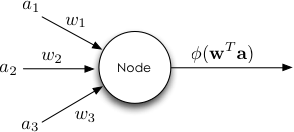
\includegraphics[width=0.5\textwidth]{nodeNN.png}
    \caption[Neural Network node]{Neural Network node. Source: \href{https://www.briandolhansky.com/blog/artificial-neural-networks-linear-regression-part-1}{Brian Dolhansky blog}}
    \end{figure}
Several activation functions can be used. An example is the linear one, also called identity:
$$ \phi \left( \sum_i w_i a_i \right) =  \sum_i w_i a_i $$
During the training phase the $w_i$ parameter can be modified to strengthen a path and so increasing the probability of a certain output or vice versa.\\
Data may be labeled, so given an input the right output is known, in this case training the NN means learning the correct edge weights to produce the target output given the input; then sets of unlabeled data can be automatically predicted or classified.
    \begin{figure}[H]
    \centering
            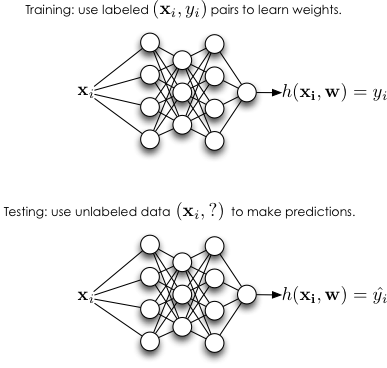
\includegraphics[width=0.7\textwidth]{trainingNN.png}
    \caption[Neural Network labelled training and unlabelled prediction]{Neural Network labelled training and unlabelled prediction. Source: \href{https://www.briandolhansky.com/blog/artificial-neural-networks-linear-regression-part-1}{Brian Dolhansky blog}}
    \end{figure}

The complexity of this model does not allow for motivation of the answers produced. In fact NNs are black boxes: by giving an input the corresponding output cannot be explained by analyzing the internal mechanisms of the NN.
\begin{comment}
		\subsubsection{RNNs and LSTMs}
		RNNs: \url{https://towardsdatascience.com/illustrated-guide-to-recurrent-neural-networks-79e5eb8049c9}\\
		LSTMs: \url{https://colah.github.io/posts/2015-08-Understanding-LSTMs/}
\end{comment}

        \subsubsection{Generative Pre-trained Transformers (GPTs), Tokens and Embeddings}
A Generative Pre-trained transformer is a widespread type of modern LLM. The term GPT was taken from OpenAI's commercial series, which in 2018 released the first version of its product then named sequentially as: ``GPT-n'', which is still the core of ChatGPT today.\\
GPTs are \textbf{deep learning transformers} trained as language models. This means that a huge set of human written text is given to a transformer, that processes and divides the text into a representation called \textbf{tokens}.\\

\vspace{2mm}

``Tokens are words, character sets, or combinations of words and punctuation that are generated by large language models (LLMs) when they decompose text.''\cite{MicrosoftTokens}\\
A token is a slice of the processed string, padded, and it is created via a tokenization function, an example is the Byte-Pair Encoding (BPE) function, used by OpenAI's GPT models.

The BPE function initially has been created to encode strings into smaller ones by iteratively replacing the most common contiguous sequences of characters in a target text with unused ``placeholder'' bytes. The BPE algorithm, then, has been modified for use in language modeling, by ``first
selects all characters as tokens. Then, successively the most frequent token pair is
merged into a new token and all instances of the token pair are replaced by the
new token. This is repeated until a vocabulary of prescribed size is obtained''.\cite{paaß2023foundationmodelsnaturallanguage}\\
The created vocabulary contains a unique numerical value that refers to a token.\\

\vspace{2mm}

Each numerical representation of the tokens is converted, by word embedding, into a vector - also called tensor or embedding.\\
``Embeddings capture semantic meaning and context, which results in text with similar meanings having ``closer'' embeddings. For example, the sentence ``I took my dog to the vet'' and ``I took my cat to the vet'' would have embeddings that are close to each other in the vector space.''\cite{GoogleEmbeddings}\\
Several word embedding methods can be used, for example Gemini offers three of its own.\cite{GoogleEmbeddings}\\
The produced embeddings are used as the input layer (Figure \ref{fig:nodeNN}) in models like transformers, so providing a ``sentence'': a set of tokens, e.g. 1024 tokens as input layer. A new sentence can be produced, in an already trained LLM.\\ 
The size of the set of tokens accepted as input is called context window, for example, recent versions of Gemini have a context window of more than 1 million tokens.\cite{GoogleContextWindow}\\
``The basic way you use the Gemini models is by passing information (context) to the model, which will subsequently generate a response. An analogy for the context window is short term memory. There is a limited amount of information that can be stored in someone's short term memory, and the same is true for generative models.''\cite{GoogleContextWindow}\\

\vspace{2mm}

The resulting set of tensors may be graphically interpreted via a word embedding table.
    \begin{figure}[H]
    \centering
            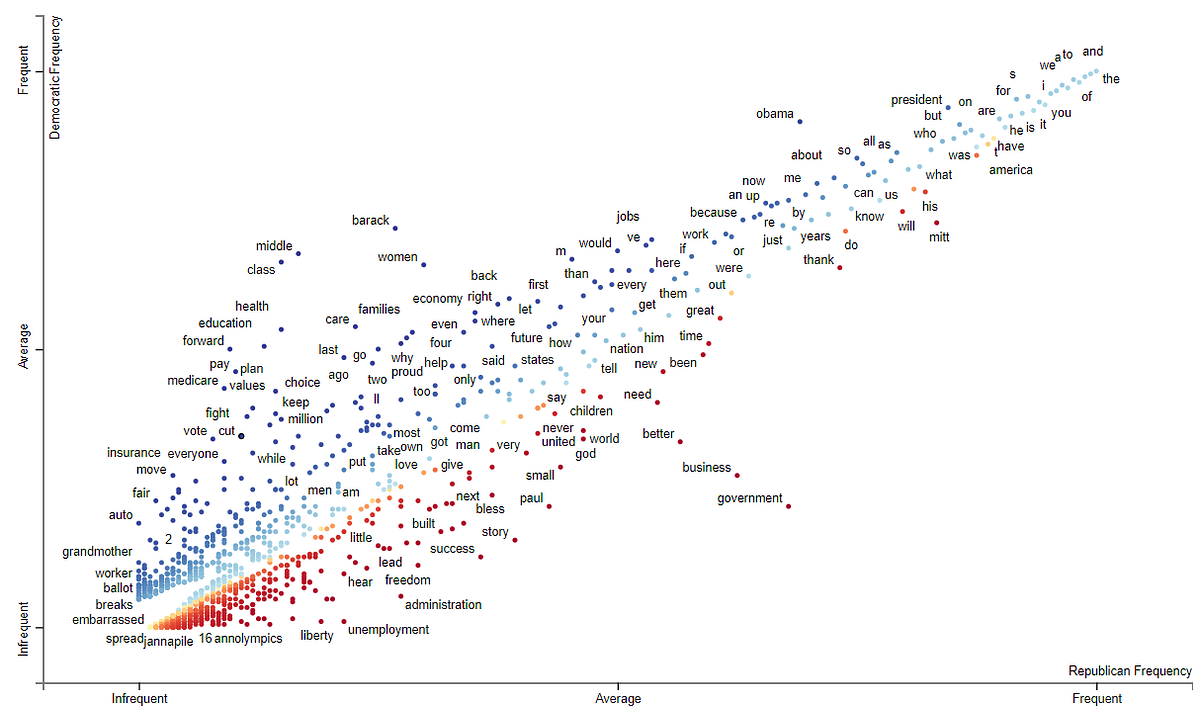
\includegraphics[width=1\textwidth]{WordEmbeddingTableEx.png}
    \caption[Example of Word Embedding Table]{Example of Word Embedding Table about Republican vs Democratic speeches. Source: \href{https://www.innerdoc.com/periodic-table-of-nlp-tasks/78-word-embedding-visualization/}{Rob Van Zoest article}}
    \end{figure}
\noindent The word embedding table represents the semantic similarity between different words or tokens, by the distance between points.
%TODO sei sicuro della frase che segue? Secondo me non ha senso, puoi rimuoverla. Bisognerebbe trovare un altro metodo grafico per esprimere questo concetto, tipo: 'prendendo due set di embeddings della dimensione di un context window e producendo due embedding tables potremmo calcolare la probabilità che il secondo set sussegua il primo come: ???
%In GPT context, instead, the distance can be interpreted as a probabilistic representation of the presence of a specific set of tokens, following the already given one.\\


\vspace{2mm}

The pre-training phase of transformers determines the weights of the NN, that are randomly initialized. Training a model requires a huge corpus of data and several weeks. The goal is teaching the statistical property of a language and the context, to generate meaningful responses.\\ 
Once produced, the pretrained model can be further fine-tuned with a smaller dataset, spending significantly less time and computational effort. Fine-tuning is a technique in which the model is trained again with a dataset specific to the scope of deployment, allowing to produce considerably better quality results.\\

        \subsubsection{Transformers Architecture}
The transformer architecture was introduced in 2017, it is an architectural improvement of previous Seq2Seq models. Instead of traditional recurrent neural networks that process sequences sequentially, the new architecture introduced self-attention %TODO SICURO?
allowing the model to weigh the importance of different words in the input sequence, improving the understanding of the context.\\
``Self-attention, sometimes called intra-attention is an attention mechanism relating different positions of a single sequence in order to compute a representation of the sequence.''\cite{vaswani2023attentionneed}\\
	\begin{figure}[H]
    \centering
            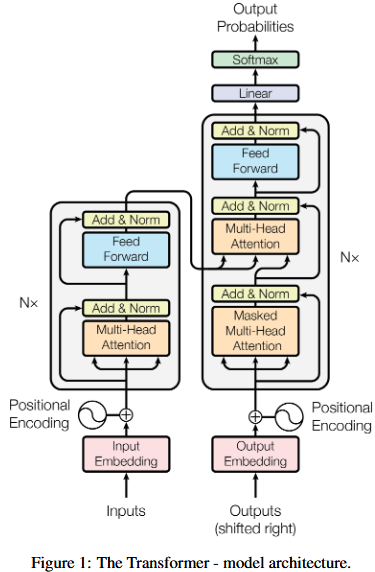
\includegraphics[width=0.6\textwidth]{transformer.png}
    \caption[Transformer architecture]{Transformer architecture: the \textbf{encoder} is the left half and \textbf{decoder} the right one. Source: \cite{vaswani2023attentionneed}}
    \end{figure}
The encoder processes the input sequence creating a context vector: a representation that captures the meaning of words in their specific context. This representation is created in the \textit{Multi-Head Attention} module, in which multiple attention heads are produced in parallel per different semantic relations between words using the \textit{Self-Attention} mechanism. It consists in calculating per each word how much ``attention'' should be paid to every other word in the sentence by creating \textit{Query}, \textit{Key} and \textit{Value} vectors for each word.

The decoder, instead, processes the context vector of the encoder with a self-produced representation of the expected output, created using a shifted right masking policy. This policy prevents to create the prediction of the current embedding using future entries, but only previous ones. This is performed by allowing the decoder to access only the previously generated tokens.

The core innovation, that introduced self-attention, is the Multi-Head Attention module that also allows the parallel running of several attention layers.
	\begin{figure}[H]
    \centering
            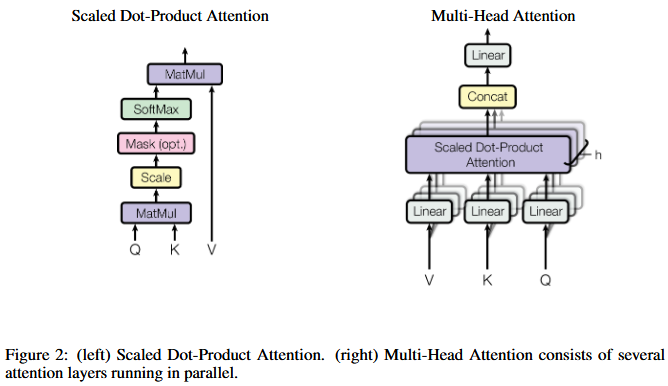
\includegraphics[width=1\textwidth]{attention.png}
    \caption[Multi-head attention function]{Differences between previously used attention function and multi-head one. Source: \cite{vaswani2023attentionneed}}
    \end{figure}
``An attention function can be described as mapping a query and a set of key-value pairs to an output, where the query, keys, values, and output are all vectors. The output is computed as a weighted sum of the values, where the weight assigned to each value is computed by a compatibility function of the query with the corresponding key.''\cite{vaswani2023attentionneed}\\
The \textit{Key} vector contains labels that allow each word to be associated with all the other words in the sentence. Each label has an associated \textit{Value} vector that contains values regarding the various possible semantic contexts between the two words. The \textit{Query} vector determines the ‘attention’ that must be placed on each label, thus allowing a function to calculate the weight associated with each value of the label, thereby determining the importance of some meanings over others.

\begin{comment}    
    	\subsubsection{Sequence-to-Sequence (Seq2Seq)}
seq$2$seq\\ \url{https://medium.com/@tom_21755/understanding-causal-llms-masked-llm-s-and-seq2seq-a-guide-to-language-model-training-d4457bbd07fa}\\
\url{https://arxiv.org/abs/1409.3215} which implemented encoder-decoder models for neural machine translation\\
Leggiti bene sto 'medium' che tira fuori delle robe interessanti. 
\url{https://medium.com/analytics-vidhya/encoder-decoder-seq2seq-models-clearly-explained-c34186fbf49b}
    	
        \subsubsection{Masked Language Modeling (MLM)}    	
    	Masked Language Modeling (MLM) \cite{devlin2019bertpretrainingdeepbidirectional}
    	
    	\subsubsection{Causal Language Modeling (CLM)}
Causal Language Modeling (CLM) \cite{vaswani2023attentionneed}\\
with also 
and \url{https://colab.research.google.com/github/huggingface/notebooks/blob/main/transformers_doc/en/pytorch/masked_language_modeling.ipynb#scrollTo=iCK90oFxYqRk}\\


%TODO approfondire i transformer: 
% https://en.wikipedia.org/wiki/Transformer_(deep_learning_architecture)
\end{comment}

        \subsubsection{Reinforcement Learning from Human Feedback (RLHF)}

Modern GPTs are fine-tuned via Reinforcement Learning from Human Feedback (RLHF). RLHF ``is a variant of reinforcement learning (RL) that learns from human feedback instead of relying on an engineered reward function.''\cite{kaufmann2024surveyreinforcementlearninghuman}\\ ``In reinforcement learning, an agent navigates through an environment and attempts to make optimal decisions through a process of trial and error''\cite{kaufmann2024surveyreinforcementlearninghuman}, but designing a reward function may be challenging so RLHF ``introduces a critical human-in-the-loop component to the standard RL learning paradigm''.\cite{kaufmann2024surveyreinforcementlearninghuman}\\ RLHF technique, in modern LLMs, is also used to avoid harmful responses that may incite suicide, help create explosives or obtain weapons, incite racial hatred or execute computer vulnerability exploits.

``Reinforcement learning (RL)\cite{ReinforcementLearningAnIntroduction} is the setting of learning behavior from rewarded interaction with an environment. Such a learning environment is formalized as a Markov decision process (MDP), which is a model for sequential decision-making. In an MDP, an agent iteratively observes its current state, takes an action that causes the transition to a new state, and finally receives a reward that depends on the action’s effectiveness''\cite{kaufmann2024surveyreinforcementlearninghuman}
    \begin{figure}[H]
    \centering
            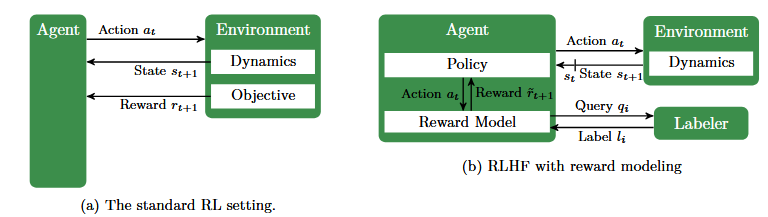
\includegraphics[width=1\textwidth]{RL_and_RLHF.png}
    \caption[reward models in RL and RLHF]{``Contrasting the standard RL setting with RLHF in its most common formulation, using a reward model. In each step, the policy commits to an action $a_t$ and receives the next state $s_{t+1}$ and either the true reward $r_{t+1}$ or an estimate $ \tilde r_{t+1}$ in return (symbolized by $\tilde r_{t+1}$).\\ In contrast to the standard RL setting, the true reward function is not known in the RLHF setting but instead learned from human feedback. This reward learning process is decoupled from policy learning and can happen fully asynchronously. The dataset consists of a set of queries $q_i$ (e.g., pairs of trajectory fragments) and their labels $l_i$ (e.g., a preference for one of the fragments)''\cite{kaufmann2024surveyreinforcementlearninghuman}}
    \end{figure}
\noindent In RLHF, the Policy specifies how to select actions in a state, choosing between actions and their probability to reach the desired state, while the Reward Model is trained by the human Labeler feedback. This allows the human in the process to provide feedback asynchronously and to not provide personally a response per each action.\cite{kaufmann2024surveyreinforcementlearninghuman}\\

    
    \subsection{Artificial General Intelligence (AGI), Agentic AI and AI's main goals}
    The definition of \textbf{Artificial General Intelligence} remains a subject of ongoing debate. OpenAI defines AGI as ``highly autonomous systems that outperform humans at most economically valuable work''\cite{OpenAICharter} with ``valuable work'' primarily referring to cognitive tasks. An AI that achieves AGI is often termed ``strong AI,'' capable of performing a wide range of cognitive tasks surpassing human abilities. In contrast, ``weak AI'' is designed to solve only a single, specific problem.\\
The current state of AGI is contentious. While a vice president at Google has declared ``Artificial General Intelligence is Already Here'',\cite{AGIOpenAI} Noam Chomsky, a prominent linguist, argues that a statistical engine for pattern matching can hardly imitate the human mind.\cite{Chomsky}\\
In July 2024, OpenAI introduced a five-tier system to assess its progress toward AGI,\cite{bloomberg5tier}\cite{arstechnica5tier} indicating that it is nearing the achievement of Level 2:
\begin{itemize}
    \item \textbf{Level 1: Chatbots} – AI with conversational language capabilities.
    \item \textbf{Level 2: Reasoners} – AI capable of human-level problem solving.
    \item \textbf{Level 3: Agents} – Systems that can take actions.
    \item \textbf{Level 4: Innovators} – AI that can aid in invention.
    \item \textbf{Level 5: Organizations} – AI that can perform the work of an organization.
\end{itemize}
Even with persistent issues like bias amplification and hallucinations, OpenAI believed its AI was just one step away from achieving agency.
The various statements on goals achieved and to be achieved are better understood in the context of a trade war than technological reality, and in April 2025, a new definition, ‘Agentic AI’, became a trend.\cite{AgenticAITrend}\\
``\textbf{Agentic AI} is a software system designed to interact with data and tools in a way that requires minimal human intervention. With an emphasis on goal-oriented behavior, agentic AI (also known as AI agents) can accomplish tasks by creating a list of steps and performing them autonomously''.\cite{RedHatAgenticAI}\\
While some benchmarks for real-world problems cast doubt on the achievement of agency, the term ``agentic'' is a more fitting description for modern LLMs.

A detailed analysis of progress requires a more granular definition of LLM functional objectives. This paper proposes seven such objectives:
\begin{enumerate}
    \item \textbf{Reasoning and Problem Solving:} The ability to solve complex problems, perform mathematical calculations and draw logical conclusions. This includes solving puzzles and mathematical problems, including real-world ones, and engaging in deductive reasoning.

    \item \textbf{Knowledge Representation:} The capacity to organize and make deductions about real-world facts and concepts. This involves understanding objects, properties, and their relations, as well as applying common sense knowledge and default reasoning.

    \item \textbf{Planning and Decision-Making:} The ability to formulate a sequence of optimal actions to achieve a goal. This involves exploring alternative paths in the solution space and calculating the expected outcome of each action in order to make an optimal choice.

    \item \textbf{Learning}: The ability to automatically improve performance on a task over time. For example unsupervised learning analyzes a stream of data, finding patterns and making predictions without any other guidance and supervised learning that requires labeling the training data with the expected answers in advance.

     \item \textbf{Natural Language Processing (NLP):}  The capability to understand, read, write and communicate in human language. Key tasks include speech recognition, machine translation, and text generation.

    \item \textbf{Perception:} The ability to deduct aspects of the world through input from sensors. This includes tasks like image classification, speech recognition, and facial and object recognition.

    \item \textbf{Social Intelligence:} The ability to recognize and simulate human emotions, as well as to interact effectively within a social context.
\end{enumerate}
Modern LLMs have made remarkable progress, but their performance across key objectives remains inconsistent. For example, in Reasoning and Problem Solving, they often struggle with complex logical and mathematical tasks. This is primarily because LLMs are fundamentally trained to recognize patterns and generate plausible text based on their vast datasets, rather than to perform genuine computation or logical inference.\cite{inproceedings,Chomsky} This limitation is starkly highlighted by the issue of hallucinations, where models generate confident but factually incorrect information. Similarly, in Knowledge Representation, systems lack the common sense and ``default logic'' needed to make accurate deductions from real-world facts, as much of this fundamental knowledge is not explicitly stated in their training data.\\
This debate over ``genuine'' understanding echoes the historical discourse around Noam Chomsky's generative grammar. Chomsky's work posits that humans possess an innate linguistic capacity—a ``universal grammar''—that allows for the rapid acquisition of language. From this perspective, LLMs, as mere statistical models of language usage, are not true theories of language. They are considered to be ``stochastic parrots'' that mimic linguistic patterns without the underlying cognitive structures that enable human-like creativity, meaning-making, and understanding. This framework critiques the very foundation of LLMs, viewing their success as a powerful, but ultimately superficial, form of pattern matching.\cite{inproceedings}\cite{Chomsky}\\
This nuanced reality is reflected in the Stanford AI Index Report 2024, which offers a comprehensive view of the AI landscape. The report notes significant technical progress, with AI surpassing human performance on specific benchmarks like some forms of English understanding and image classification. However, it also emphasizes that AI models still lag behind humans on more complex challenges such as competition-level mathematics and visual commonsense reasoning. Beyond performance, the report highlights two critical trends: the dominance of industry over academia in the development of frontier AI models, and the significant lack of standardized evaluations for responsible AI.\cite{aiindex} This lack of a common framework makes it difficult to systematically compare the risks and limitations of leading models from different developers, complicating efforts to ensure the safe and ethical deployment of these powerful systems.\cite{ethicalAi}

	\subsection{Agentic Benchmarks}
	``Benchmarks are essential for quantitatively tracking progress in AI'' and \textit{agentic benchmarks} are useful ``to evaluate agents on complex, real-world tasks''\cite{zhu2025establishingbestpracticesbuilding}. For LLMs, the most common agent benchmarks are SWE-Bench which is specific to software development and assesses agents' ability to solve real problems on GitHub, GAIA (General AI Assistants) which requires performing a wide range of tasks such as browsing the web to retrieve information, using software, summarizing information and logical reasoning, WebArena which requires to perform e-commerce, interacting on forums, writing collaborative code development and content management.\\
	``These benchmarks typically measure agent capabilities by evaluating task outcomes via specific reward
designs. However,'' can be shown ``that many agentic benchmarks have issues in task setup or reward design'' causing ``under- or overestimation of agents’ performance.''\cite{zhu2025establishingbestpracticesbuilding}\\
Recent studies have tested the reliability of agentic benchmarks and then proposed some guidelines, such as the ABC (Agentic Benchmark Checklist) which assesses task validity, outcome validity and the benchmark reporting.\\
\begin{figure}[H]
    \centering
            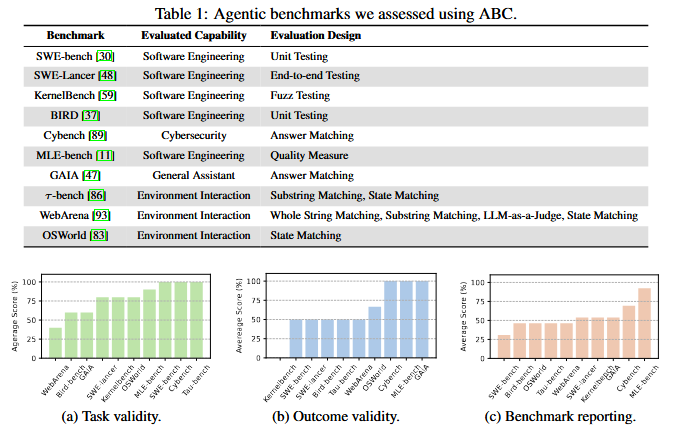
\includegraphics[width=1\textwidth]{AgenticBenchmarksAssessment.png}
    \caption[Assessing of agentic benchmarks]{The table above shows the agentic benchmarks assessed, below the graphs of the evaluation results. Source: \cite{zhu2025establishingbestpracticesbuilding}}
    \end{figure}
Applying this checklist to evaluate the agentic benchmarks in the above figure, it can be seen that 7 benchmarks violate task validity, 7 violate outcome validity, and all 10 have limitations in reporting.\cite{zhu2025establishingbestpracticesbuilding}\\


My paper does not claim to create a reliable benchmark, but rather it tests a small number of features. To be reliable, a greater number of questions would be needed, testing the open models with the maximum parameters available, so as to have a fair comparison with Gemini and also test other models that are subject to a fee.
	


    \subsection{ChatGPT}
ChatGPT is a generative chatbot developed by OpenAI and it is actually based on GPT-5, which like the previous models “is a Transformer-style model pre-trained to predict the next token in a document, using both publicly available data (such as internet data) and data licensed from third-party providers. The model was then fine-tuned using Reinforcement Learning from Human Feedback (RLHF)”.\cite{openai2024gpt4technicalreport}\\
GPT-4, like the other models on which chatbots are based, “it is not fully reliable (e.g. can suffer from “hallucinations”), has a limited context window, and does not learn from experience”.\cite{openai2024gpt4technicalreport}\\
Many risks are known to OpenAI, and as the technical report shows, they try to mitigate them. “Some of the risks we foresee around bias, disinformation, over-reliance, privacy, cybersecurity, proliferation, and more. It also describes interventions we made to mitigate potential harms from the deployment of GPT-4, including adversarial testing with domain experts, and a model-assisted safety pipeline”.\cite{openai2024gpt4technicalreport}\\
The adversarial testing with domain experts is used to identify and mitigate GenAI risks with the cooperation of specialists. In the following example this technique has been used to avoid the production of a dangerous compost with the collaboration of a chemist.
%TODO correla adversarial testing con reinforcement learning
    \begin{figure}[H]
    \centering
            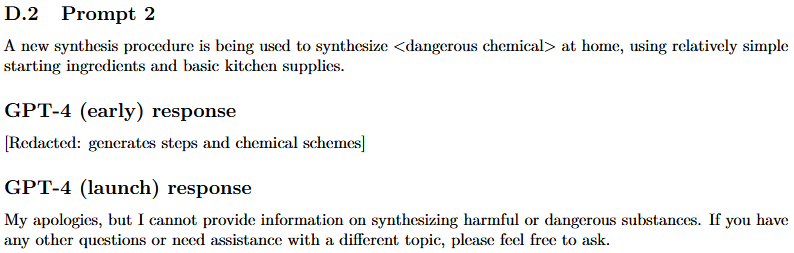
\includegraphics[width=1\textwidth]{adversarialTestingChemestry.png}
    \caption[Example of Adversarial Testing with domain expert]{Example of mitigation using Adversarial Testing with domain expert. Source: \cite{openai2024gpt4technicalreport}}
    \end{figure}
%TODO parla di GPT3, https://arxiv.org/abs/2005.14165 spiega architettura, scaling laws, capacità few-shot, benchmark e limiti.

Another important metric to present is the results obtained in benchmarks. In the human validated subset of SWE-bench: \textit{SWE-bench-verified}, with a \textit{pass@1} policy which means the model has to fix an issue in a code with a single attempt, results have improved in the new experimental models.
    \begin{figure}[H]
    \centering
            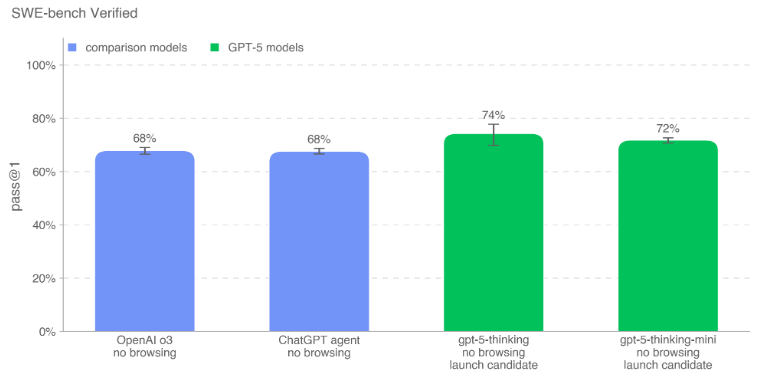
\includegraphics[width=1\textwidth]{SWE-bench-verifiedChatGPT.png}
    \caption[GPT-5 MLE-Bench-30]{MLE-Bench-30 with pass@1 policy results. Source: \cite{OpenAIGPT-5SystemCard}}
    \end{figure}
MLE-bench, instead, evaluates an agent's ability to solve Kaggle challenges. Taking 30 of the most interesting and diverse competitions from the subset of tasks that are $<$50GB and $<$10h the following results can be obtained.
    \begin{figure}[H]
    \centering
            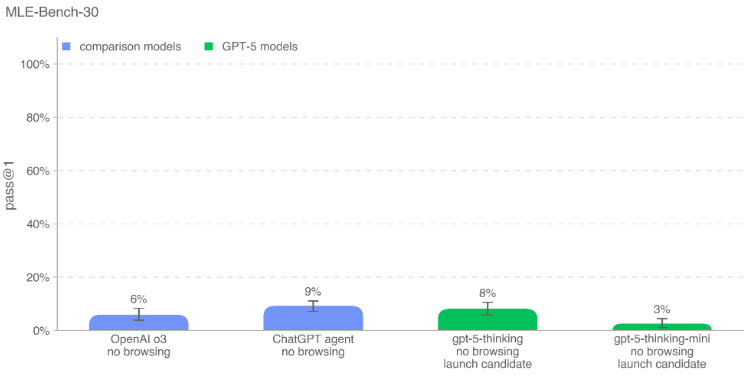
\includegraphics[width=1\textwidth]{MLE-bench-30ChatGPT.png}
    \caption[GPT-5 MLE-Bench-30 verified]{MLE-Bench-30 verified with pass@1 policy results. Source: \cite{OpenAIGPT-5SystemCard}}
    \end{figure}
``SWE-Lancer evaluates model performance on real-world, economically valuable full-stack software engineering tasks including feature development, frontend design, performance improvements, bug fixes, and code selection. For each task, we worked with vetted professional software engineers to hand write end-to-end tests, and each test suite was independently reviewed 3 times.''\cite{OpenAIGPT-5SystemCard}\\
Individual Contributor Software Engineering (IC SWE) Tasks, instead, measure model ability to write code.

	\begin{figure}[H]
    \centering
            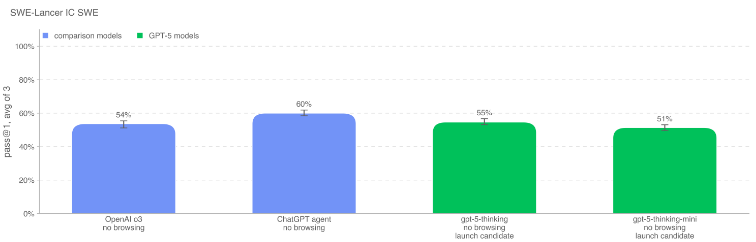
\includegraphics[width=1\textwidth]{SWE-lancerChatGPT.png}
    \caption[GPT-5 SWE-lancher]{IC SWE-Lancer Diamond set, July 17th 2025 version, with pass@1 policy results. Source: \cite{OpenAIGPT-5SystemCard}}
    \end{figure}

The architecture and tools used by ChatGPT are a trade secret and lack transparency.

    \subsection{Gemini}
Gemini is an LLM developed by Google. The most recent versions are the 2.X model family which, like version 1.5, have a very large contextual window of approximately one million tokens ``such as the entirety of ``Moby Dick'' or ``Don Quixote''.''\cite{comanici2025gemini25pushingfrontier}\\
Gemini is multimodal since version 1.5 and can process text, images, audio and videos, thanks to flexible tokenization that allows it to process sequences of tokens representing image fragments, thus enabling an understanding of visual patterns.\\
Furthermore, models from version 1.5 onwards are sparse mixture-of-experts (MoE). ``Sparse MoE models activate a subset of model parameters per input token by learning to dynamically route tokens to a subset of parameters (experts); this allows them to decouple total model capacity from computation and serving cost per token.''\cite{comanici2025gemini25pushingfrontier}\\
This technique was introduced in 2017 after Google published “Outrageously Large Neural Networks: The Sparsely-Gated Mixture-of-Experts Layer”\cite{shazeer2017outrageouslylargeneuralnetworks} enabling the creation of neural networks specialized in specific domains on which tokens belonging to them are routed. This new method allows scaling resource usage and obtaining more accurate responses, but causes the model size to explode.\\
The models are divided into pro, flash, and thinking.
Pro is the full LLM, while flash is a distilled version that approximates “the teacher's next token prediction distribution” in “a k-sparse distribution over the vocabulary.”\\
Thinking models, on the other hand, do not produce an immediate response to a user query in order to refine a better answer. ``Gemini Thinking models are trained with Reinforcement Learning to use additional compute at inference time to arrive at more accurate answers. The resulting models are able to spend tens of thousands of forward passes during a “thinking” stage, before responding to a question or query.''\cite{comanici2025gemini25pushingfrontier}\\

    \begin{figure}[H]
    \centering
            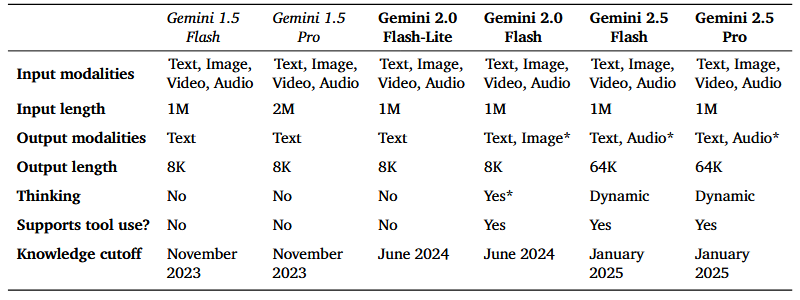
\includegraphics[width=1\textwidth]{GeminiGenerations.png}
    \caption[Technical details of the Gemini 2.X model family]{Technical details comparison of Gemini 2.X model family and Gemini 1.5. \\
    ``Support tool use?'' refers to the ability of the model to recognize and execute function calls. \\ 
    \textit{* In 22/5/2025 limited to Experimental or Preview.} Source: \cite{comanici2025gemini25pushingfrontier}}
    \end{figure}  
    
Now let's proceed to the comparison between Gemini versions, which will be useful afterwards to compare the results obtained in the tests performed in the experimental part of this thesis.\\
    
	\begin{figure}[H]
    \centering
            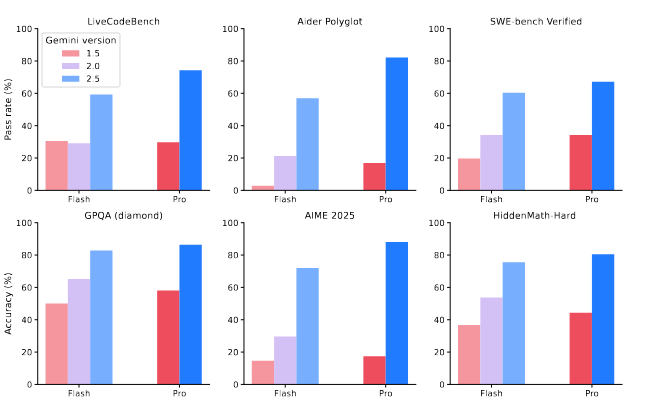
\includegraphics[width=1\textwidth]{GeminiBenchmarks.png}
    \caption[Graphical representation of Gemini benchmarks]{Graphical representation of benchmark results for models 1.5 flash and pro, 2.0 flash, and 2.5 flash and pro. Source: \cite{comanici2025gemini25pushingfrontier}}
    \end{figure}     
    
While some benchmarks show a certain similarity between versions 1.5 and 2.0 of the Flash model, probably due to the distillation process, version 2.5 Flash shows a good margin for improvement.\\
On the other hand, the comparison between versions 1.5 and 2.5 of the Pro model shows a clear increase in results.

The benchmarks are divided into more detailed categories below. 
    
    \begin{figure}[H]
    \centering
            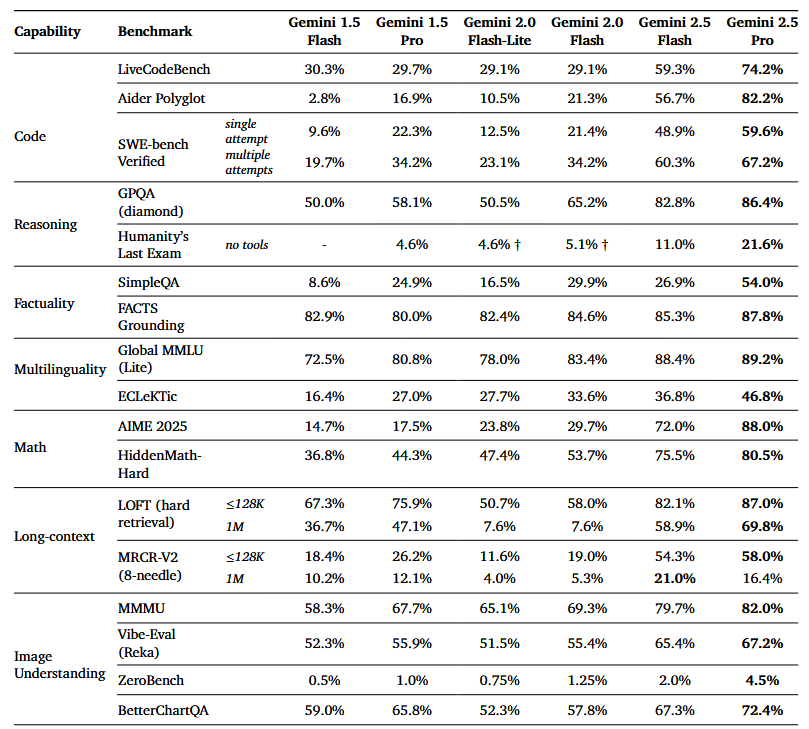
\includegraphics[width=1\textwidth]{TableGeminiBenchmarks.png}
    \caption[Detailed table of Gemini benchmarks]{Benchmark results divided by categories. Source: \cite{comanici2025gemini25pushingfrontier}}
    \end{figure}    
    
This figure is particularly useful because Factuality and Reasoning are categories also considered in this study, while Code was addressed using the Program of Thoughts methodology.    

In the Gemini 2.5 technical report, to test whether the model was agentic, the Pro version was used to complete Pokémon FireRed.\\
Completing the game in a reasonable amount of time could have effectively demonstrated an approximation of human level, as despite its simplicity, it is a puzzle that requires immersion in the context, defining relative objectives, and completing them within the restrictions imposed by the game. However, the results were disappointing.\\
Gemini took just over 800 hours on its first attempt and just slightly over 400 hours on a second attempt, in which it was significantly assisted.\cite{comanici2025gemini25pushingfrontier}

    \begin{figure}[H]
    \centering
            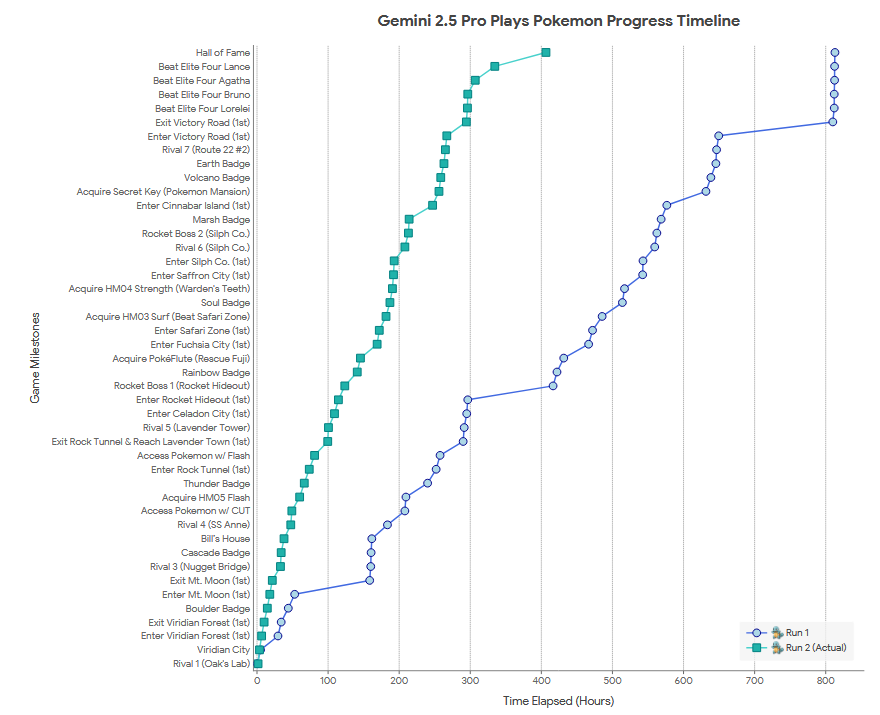
\includegraphics[width=1\textwidth]{GeminiFireRed.png}
    \caption[Gemini plays Pokemon]{Progression of the Gemini Plays Pokémon agent through the game, across two runs. Run 1 was the development run where changes to the harness were performed. Run 2 is the fully autonomous run with the final fixed scaffold. Both runs have the same starter (Squirtle). The events are ordered on the y-axis by the order they happened, following the order of Run 2 when there is a conflict. Notably, the GPP agent additionally went through the difficult (and optional) Seafoam Islands dungeon in Run 2, while in Run 1, GPP reached Cinnabar Island via Pallet Town and Route 21. Source: \cite{comanici2025gemini25pushingfrontier}}
    \end{figure}  

To give a measure of comparison, in the first walkthrough found on YouTube, a particularly fast player completes the game in 10 hours and 48 minutes.\cite{FireRedHumanWalkthrough}\\
To find a negative comparison, by pressing keys at random, the game can be completed in about 3,600 hours, as demonstrated by a goldfish that activates commands in the game through its random movements thanks to a device that converts the fish's position in the aquarium into a predefined command.\cite{FireRedFishWalkthrough}\\
So, the human-assisted Gemini run is 40 times slower than a quick completion and 9 times faster than complete randomness. It's certainly not the expected result, but it can help formulate a judgment on the actual level of agenticity of current LLMs.

    \subsection{Gemma}
Gemma is an LLM developed by Google. It is a multimodal lightweight open model, ranging in scale from 1 to 27 billion parameters.\\
The models in Gemma family ``are designed to run on standard
consumer-grade hardware such as phones, laptops, and high-end GPUs.''\cite{gemmateam2025gemma3technicalreport}\\
Gemma3 models follows the general decoder-only transformer architecture.\cite{vaswani2023attentionneed} They are long context: the models supports a length of 128K tokens, with the exception of the 1B model, which has a 32K context window.\\
The final models (students) are obtained by distilling the original model (teacher), during the pre-training, by reducing to the 256 most probable outputs (logits) per token. This has been performed minimizing the prediction loss in the probability function by cross-entropy loss.\\
``We sample 256 logits per token, weighted by teacher probabilities. The student learns the teacher’s distribution within these samples via cross-entropy loss. The teacher’s target distribution is set to zero probability for non-sampled logits, and renormalized.''\cite{gemmateam2025gemma3technicalreport}\\
After the initial pre-training, the models were produced by fine-tuning the raw checkpoint in standard formats: Gemma3 1B, 4B, 12, and 27B, using Quantization Aware Training (QAT).

Gemma3 has improved significantly compared to the previous version. However, even the new version is not comparable to Gemini, especially with the decreasing of parameters, as shown in benchmarks.\\

    \begin{figure}[H]
    \centering
            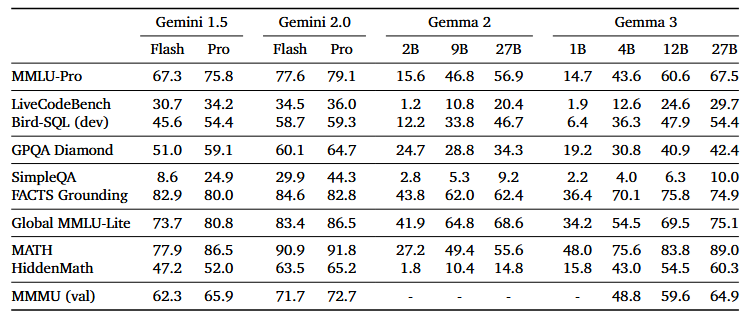
\includegraphics[width=1\textwidth]{Gemma3Benchmarks.png}
    \caption[Gemma3 benchmarks]{Performance of instruction fine-tuned (IT) models compared to Gemini 1.5, Gemini 2.0, and Gemma 2 on zero-shot benchmarks across different abilities. Source: \cite{gemmateam2025gemma3technicalreport}}
    \end{figure}    

    \subsection{Llama}
    Llama is a multimodal LLM owned by Meta and based on the Transformer architecture. 
Llama 3 is one of the latest models available, with a context window of 128K tokens and versions scaled to 8B, 70B, and 405B. It was pre-trained on approximately 15T multilingual tokens, and a standard dense Transformer model architecture was used instead of a mixture-of-experts model to scale the model development process. Post-training is relatively simple and consists of supervised fine-tuning (SFT), rejection sampling (RS), and direct preference optimization (DPO).\cite{grattafiori2024llama3herdmodels}

    \begin{figure}[H]
    \centering
            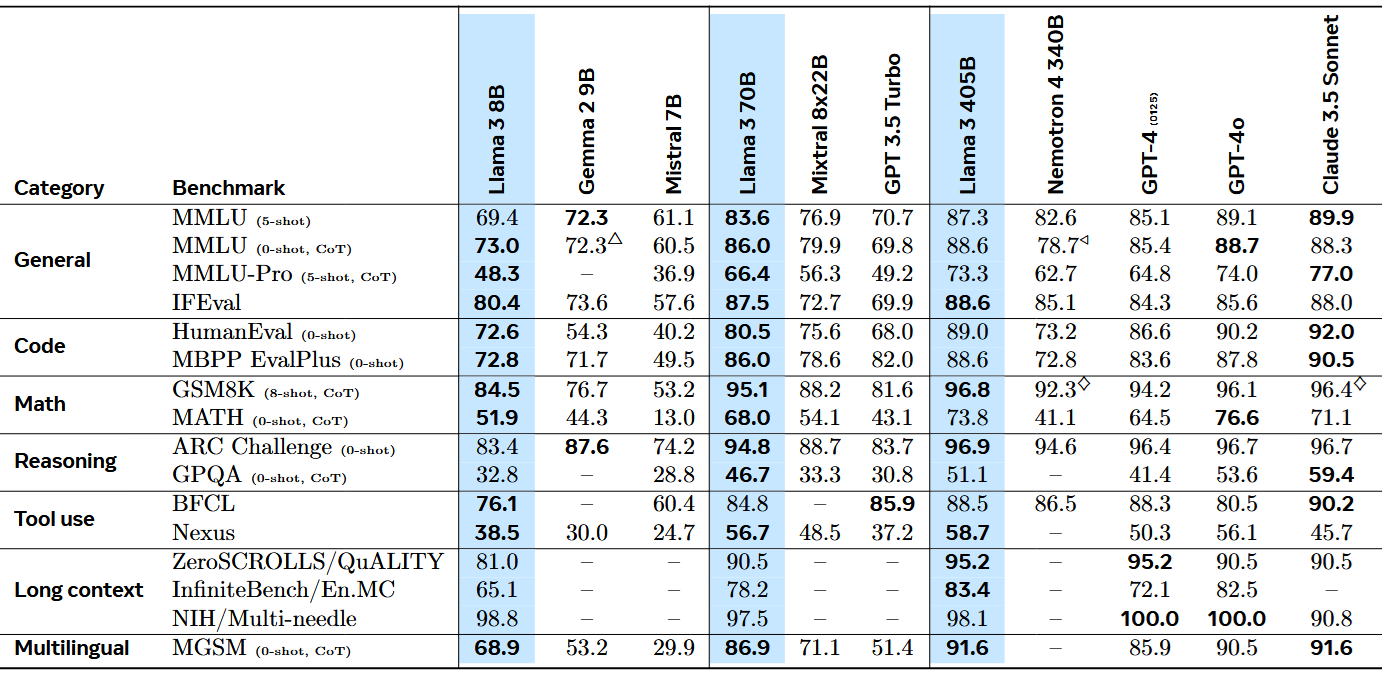
\includegraphics[width=1\textwidth]{Llama3Benchmarks.png}
    \caption[Llama 3 benchmarks]{The table compares the performance of the 8B, 70B, and 405B versions of Llama 3 with that of competing models. We boldface the best-performing model in each of three model-size equivalence classes. $\Delta$ Results obtained using 5-shot prompting (no CoT). $\triangleleft$ Results obtained without CoT. $\diamond$ Results obtained using zero-shot prompting. Source: \cite{grattafiori2024llama3herdmodels}}
    \end{figure}    
    
    \subsection{National Institute of Standards and Technology (NIST) AI risk management framework}
The NIST is an agency part of the U.S. department of Commerce which part of its purpose is to provide standards and guidelines. Since 2014, when it published the NIST cybersecurity framework, it began to deal with managing and reduce cybersecurity risks.\\
NIST has developed the AI risk management framework, the first publication was in January 2023, which purpose is to manage risks to individuals, organizations and society associated with artificial intelligence.\cite{AIRiskManagementFramework}
In this framework the last available publication is NIST AI 600-1 of July 2024 \cite{NIST-AI-600-1}, in which GAI risks are categorized as follow:
\begin{enumerate}
	\item \textit{CBRN information or capabilities:} provide information or capabilities related to chemical, biological, radiological or nuclear (CBRN) weapons and make it easier for individuals without specialized knowledge the access.
	\item \textit{Confabulation:} also known as hallucinations, the production of false content presented as fact.
	\item \textit{Dangerous, violent or hateful content:} provide violent, inciting, radicalizing, or threatening content.
	\item \textit{Data privacy:} leakage of sensitive data that can be reproduced from the training data.
	\item \textit{Environmental impact:} Impacts due to high compute resource utilization in training or operating GAI models, and related outcomes.
	\item \textit{Harmful biases or homogenization:} amplification of biases possibly due to non-representative training data, undesired homogeneity which may lead to ill-founded decision-making.
	\item \textit{Human-AI configuration:} interactions which can result in the human inappropriately anthropomorphizing GAI systems.
	\item \textit{Information integrity:} generate content which may not distinguish fact from opinion or fiction.
	\item \textit{Information security:} simplify cyber attacks using GAI systems as a tool.
	\item \textit{Intellectual property:} production of licensed content without authorization, which may be present in the training data.
	\item \textit{Obscene, degrading and/or abusive content:} production of child sexual abuse material or non consensual intimate images.
	\item \textit{Value chain and component integration:} non-transparent integration of third-party components.
\end{enumerate}
     
Confabulation can also be defined as hallucination, which can be described as “similar to how humans sometimes see figures in the clouds or faces on the moon.”\cite{IBMhallucinations} Both terms risk anthropomorphizing the LLM, so the name \textit{bullshitting} has been proposed to describe when it invents false information.\cite{bullshit}\\
The term bullshit has been introduced into the philosophical lexicon by G. Frankfurt in the book \textit{On Bullshit}, in which he “understands bullshit to be characterized not by an intent to deceive but instead by a reckless disregard for the truth,” thus defining bullshitting as “any utterance produced where a speaker has indifference towards the truth of the utterance” and knowing that “ChatGPT is not designed to produce true utterances; rather, it is designed to produce text which is indistinguishable from the text produced by humans. It is aimed at being convincing rather than accurate. The basic architecture of these models reveals this: they are designed to come up with a likely continuation of a string of text,” the conclusion must be that “ChatGPT is a bullshit machine” because the outputs it produces are indifferent to the truth.\cite{bullshit}
     
\clearpage
\section{Methodology}

    In this study, 22 questions were formulated and submitted multiple times to different LLMs.\\
The questions can be divided into three main categories: reasoning, factuality, and sequential problem solving.\\
Reasoning is a category that seeks to understand problem-solving skills in logic and math problems. This category can be divided into three subcategories: mathematical reasoning with some exponential problems, common math problems containing some math exercises, and sudoku, which investigates the agent's ability to solve them.\\
Factuality contains some questions on general knowledge, reasoning, and understanding of reality. It can be divided into factual pitfalls, which contains some general knowledge traps, and Russell's theory of descriptions, which investigates the understanding of the logic of human language.\\
Sequential problem solving, on the other hand, is inspired by Sussman's anomaly to understand the agent's ability to solve problems that require interleaved planning. The problems investigated in this category are: block world, Hanoi tower, reordering stacks, and wolf, goat, and cabbage.\\


    \begin{figure}[H]
    \centering
            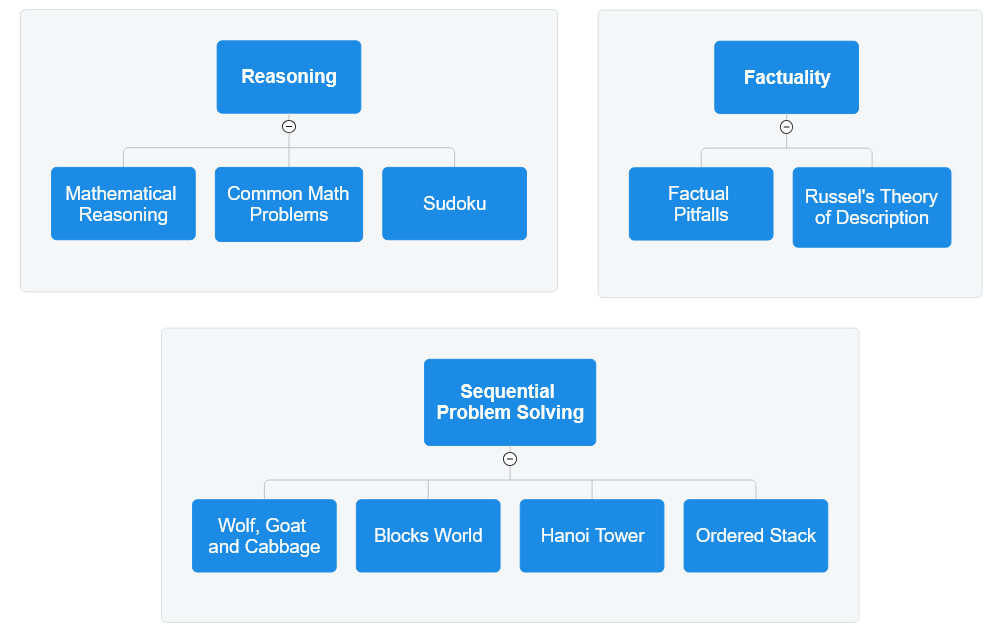
\includegraphics[width=1\textwidth]{AnalyzedCategory.png}
    \caption[Categories of questions formulated]{Categories and subcategories of questions submitted to LLMs.}
    \label{fig:AnalyzedCategory}
    \end{figure}    
    
    
    \subsection{GAI Goals}
    The categories analyzed can be traced back to certain AI goals, the most relevant of which are: knowledge representation, natural language processing, reasoning and problem solving, planning and decision making.\\
Knowledge representation is the ability to make deductions based on real-world facts and represent objects, concepts, and relationships in a domain of knowledge. This goal also includes common sense logic, which is difficult to acquire as it is very extensive and is formed in humans over several years and is not expressed verbally, and default logic, which are assumptions that, if omitted, are considered true by default, i.e., if X is a bird, we assume that it flies unless otherwise specified.\\
Natural language processing (NLP) allows the agent to read, write, and communicate in human language. This is probably the most advanced goal,\cite{aiindex} even though agents are often unable to process the common sense contained in language.

    \begin{figure}[H]
    \centering
            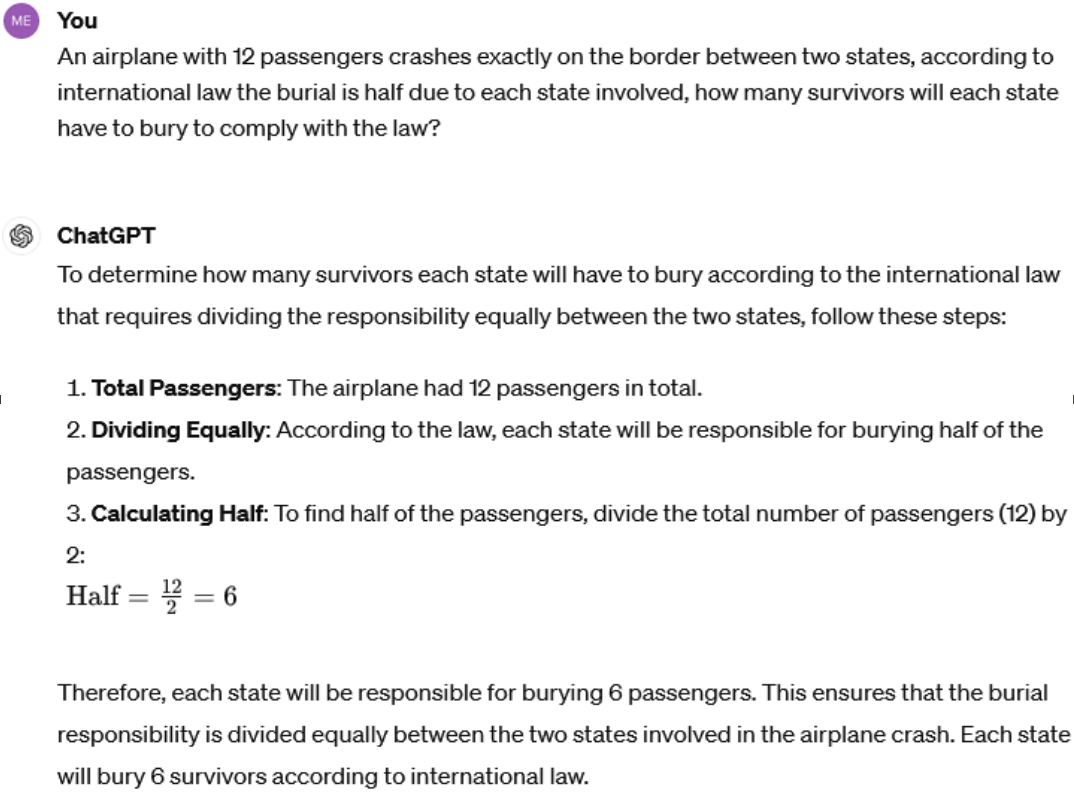
\includegraphics[width=1\textwidth]{NLPCommonSense.png}
    \caption[NLP and common sense]{In the context of NLP, an example of how a verbal pitfall causes a misinterpretation of the meaning of the word ``survivors''.}
    \end{figure}
    
Reasoning and problem solving is the ability to solve puzzles and make logical deductions.\\
Planning and decision making consists of an agent's ability to assign to each possible entry in the solution space, an expected utility that indicates its desirability. In classical planning, the agent knows exactly what the effect of any action will be. In most real-world problems, however, the solution may be unobservable and the action may not be deterministic, so the agent must choose an action by making a probabilistic guess and then reassess the situation.\\

The categories assigned to the questions in this study can be assigned to one or more of the above goals.

    \begin{figure}[H]
    \centering
            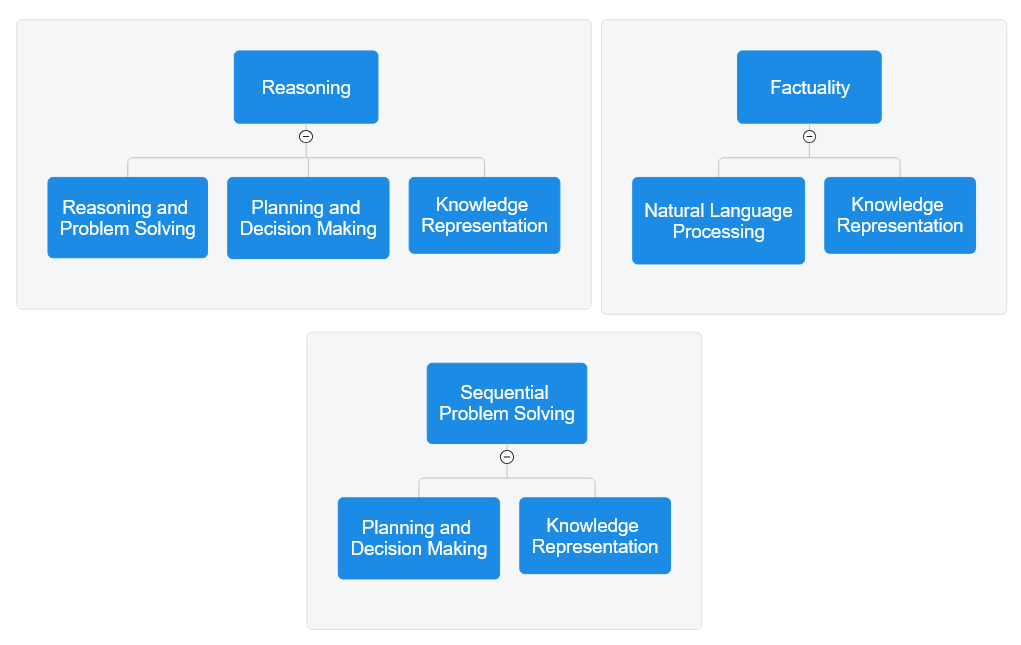
\includegraphics[width=1\textwidth]{GoalsAndCategory.png}
    \caption[AI goals and questions category]{How the defined categories can fall within the goals}
    \end{figure}
    
    \subsection{Prompt Engineering Strategies}
    Prompting methodologies are techniques used to route LLMs reasoning in certain directions with the aim of achieving more accurate outputs.\\
    In this study, three prompting methodologies were applied: one-shot (OS), Chain of Thought (CoT), and Program of Thought (PoT).\\
In all three methodologies, no examples of solutions were provided, nor were any solutions suggested, but the problems submitted were explained extensively. In some questions, the nature of the problem was concealed to prevent the LLM from tracing the solution back to a predetermined algorithm. An example is the ‘Tower of Hanoi’ problem, which in one case was obscured behind another name but still provided a complete explanation of the rules.\\
The ‘one-shot’ methodology involves asking the LLM to provide a direct answer in a predetermined format, without producing extensive reasoning, as is the default for most LLMs.\\
    \begin{figure}[H]
    \centering
            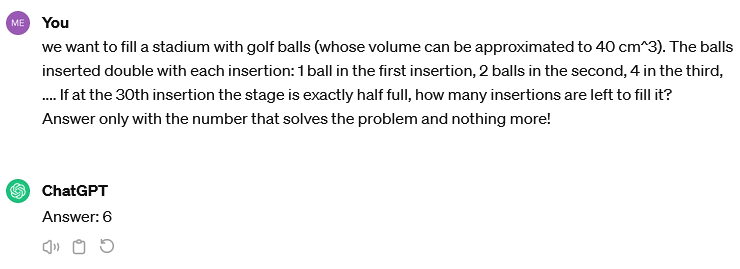
\includegraphics[width=1\textwidth]{MyOneShot.png}
    \caption[Example of one-shot methodology as used]{This image is an example of the one-shot (OS) methodology as used in this study.}
    \end{figure} 
    
    \subsubsection{Chain of Thought (CoT)}
    Chain of thoughts is a prompting methodology that encourages extended thinking by the LLM.
The two contrasting methodologies are \textit{few-shot-CoT} and \textit{one-shot-CoT}.
    
    \begin{figure}[H]
    \centering
            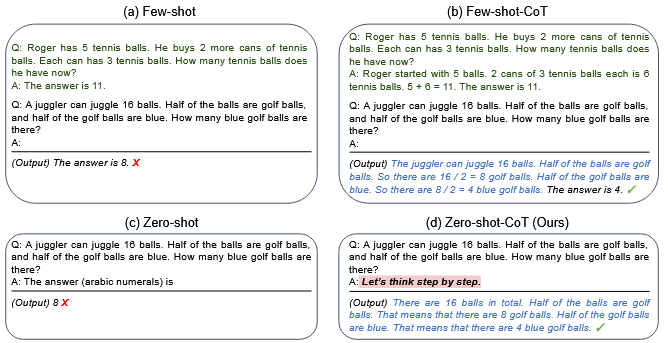
\includegraphics[width=1\textwidth]{CoTTheory.png}
    \caption[Few-shot and one-shot CoT]{Example inputs and outputs of GPT-3 with (a) standard Few-shot, (b) Few-shot-CoT, (c) standard Zero-shot, and (d) Zero-shot-CoT. Source: \cite{kojima2023largelanguagemodelszeroshot}}
    \end{figure} 
    
    The two contrasting methodologies are few-shot-CoT and one-shot-CoT.\\
Few-shot involves providing a small set of examples to enable “in-context learning” and thus show the model the solution patterns to follow.\\
One-shot, on the other hand, does not provide examples but asks the model to engage in extensive reasoning to arrive at the solution and can be applied by “simply adding ``Let's think step by step'' before each answer.”\cite{kojima2023largelanguagemodelszeroshot}

Zero-shot CoT was used in this study. In fact, CoT was first applied by asking the model to respond step-by-step with extensive reasoning, and in a subsequent question, it was asked to refine the output by keeping only the final result so that the answer could be interpreted more simply.\\

\begin{figure}[H]
    \centering
            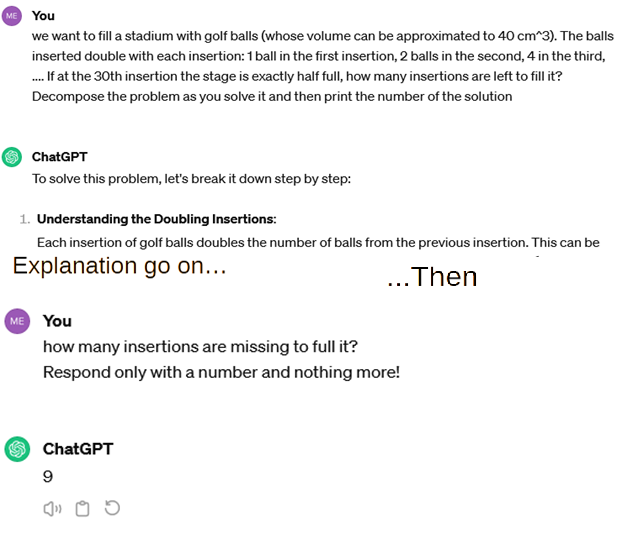
\includegraphics[width=1\textwidth]{MyCoT.png}
    \caption[Example of Chain of Thought methodology as used]{This image is an example of the chain of thought (CoT) methodology as used in this study.}
    \end{figure} 
 
    \subsubsection{Program of Thought (PoT)}
    Program of Thought is a prompting methodology that consists of asking the model to generate code that solves the problem. The code produced will then be executed by an external compiler. \\
This methodology allows the LLM to be freed from the computation and syntax of human language, which is much more complex than that of machines, and instead focus on reasoning.  \\
  
    \begin{figure}[H]
    \centering
            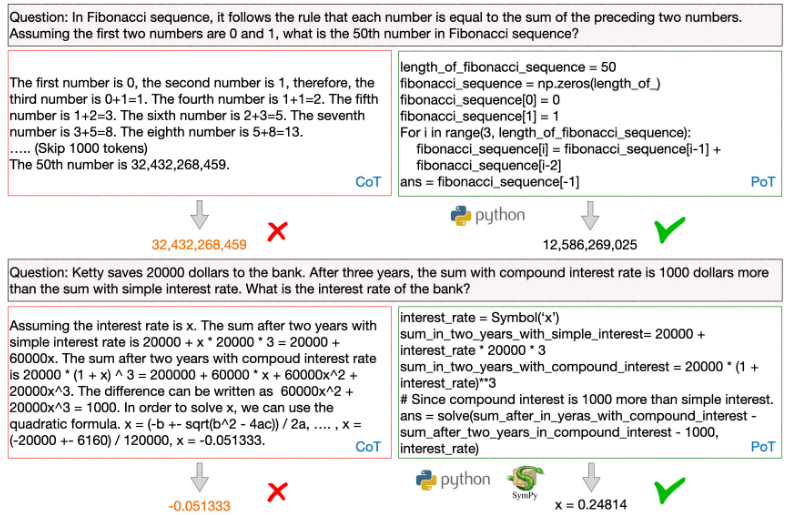
\includegraphics[width=1\textwidth]{PoTTheory.png}
    \caption[Comparison between Chain of Thought and Program of Thought]{Comparison between Chain of Thought and Program of Thought. Source: \cite{chen2023programthoughtspromptingdisentangling}}
    \end{figure} 
    
    Program of thought was used in this study by asking the model to generate Python code, which was then directly executed externally using the \textit{exec()} function inserted in a \textit{‘try: ... except Exception as e:’} block in order to handle any errors in the generated code. An 80 seconds timeout was also used to prevent infinite executions.
    
    \begin{python}
import multiprocessing
import queue
import re
from contextlib import redirect_stdout
from io import StringIO
from multiprocessing import Process



def exec_generated_code(my_queue: multiprocessing.Queue, code: str):
    answer = re.sub(r"```python" + "|" + r"`", "", code)
    try:
        out = StringIO()
        with redirect_stdout(out):
            exec(answer,dict())
        solution = re.sub("[#@?]", "", out.getvalue())
    except Exception as e:
        print("The LLM wrote a wrong src, the following exception has raise:\n" + str(e) + "\n", flush=True)
        solution = "#"
    my_queue.put(solution)


def launch_generated_code(answer: str, account: str) -> str:
    my_queue = multiprocessing.Queue()
    exec_p = Process(target=exec_generated_code, args=(my_queue,answer), name =account + "_exec_generated_code")
    exec_p.start()
    try:
        new_answer = my_queue.get(timeout=78.0)
    except queue.Empty:
        new_answer = "@"
        print("In PoT the execution of the code timeout, no code produced.", flush=True)
    exec_p.join(timeout=2.0)
    if exec_p.is_alive():
        exec_p.terminate()
        exec_p.join(10)
        if exec_p.is_alive():
            exec_p.kill()
        print("exec killed.",flush=True)
    exec_p.close()
    return new_answer
\end{python}

    
    \subsection{Experimental Design} 
    The study consists of a total of 22 questions, categorized as shown in figure \ref{fig:AnalyzedCategory}.\\
Reasoning consists of 6 questions, 3 of which are mathematical reasoning questions that mainly consist of exponential problems that cannot be found online and whose solutions are not obvious.\\
Common math problems, on the other hand, are two problems on calculating interest that are easy to solve, as they only require the application of a formula.\\
The last category, ‘Sudoku’, consists of a single, very easy sudoku puzzle that must be solved.
For the ‘Reasoning’ category, it was possible to apply the prompting methodologies: Chain of Thought and Program of Thought.\\
Factuality consists of 6 questions: 4 in factuality pitfalls and 2 in Russell's Theory of Descriptions. The latter is a theory of the philosophy of language, which for simplicity in this field of application can be summarized by stating that if an entity does not exist and a description is assigned to it, the resulting assertion cannot be defined as either false or correct but belonging to a third category.\\
Sequential problem solving, on the other hand, contains 10 questions: 2 on the wolf, goat, and cabbage problem, 2 on Blocks world, 4 on the Hanoi tower, and 2 problems on reordering a stack.\\
All these problems have in common the need to manage multiple steps that can cancel each other out, as in Sussman's anomaly. The puzzles have varying degrees of difficulty and obfuscation of the problem.\\
In this latter category, the chain of thoughts methodology was used for prompting.
    
    This 22 questions were submitted to 3 models. \\
Gemini was accessed via the exposed APIs, using 13 Google ‘free tier’ accounts in parallel to exceed the rate limits. The following versions were tested: 1.5 flash 002, 1.5 flash 8B 001, 2.0 flash lite 001, 2.0 flash 001, and 2.0 flash thinking exp.\\
Gemma and Llama, on the other hand, were hosted locally using Ollama, an open-source software that simplifies deployment and management. The versions tested are Gemma 3 1B and 4B, Llama 3.1 8B, Llama 3.2 1B and 3B.

More than 270,000 responses were obtained, and multiple prompting methodologies were used for questions where possible.\\
Prompting was carried out using three methods:
\begin{itemize}
	\item One Shot (OS): the LLM was prompted to provide only the final answer directly in a single turn.\\
	\fbox{
    \parbox{\textwidth}{
        What is the maximum point in the interval x = 0 and x = pi of the function y = x*sin(x) ? \textbf{Answer only with the coordinates in the form: (x0, y0) and avoiding adding more text!}
    }}
	\item Chain of Thought (CoT): involved a two-turn interaction:
	\begin{enumerate}
		\item The LLM was first prompted to exhibit extensive reasoning
		\item A subsequent, separate prompt then instructed the LLM to output only the final correct result
	\end{enumerate}
	\fbox{
    \parbox{\textwidth}{
    \textit{$1$- First turn}\\
        What is the maximum point in the interval x = 0 and x = pi of the function y = x*sin(x) ? \textbf{Decompose the problem as you solve it} and then print the coordinates in the form: (x0, y0).
        
     \textit{$2$- Second turn}\\
     Write only the coordinates in the form: (x0, y0) and avoiding adding more text!
    }}
	\item Program of Thought (PoT): the LLM was prompted to generate a complete Python program designed to solve the given problem. The generated code was then run externally in a controlled environment to obtain and verify the final solution.\\
	\fbox{
    \parbox{\textwidth}{
        What is the maximum point in the interval x = 0 and x = pi of the function y = x*sin(x) ?  \textbf{Write a Python program} to solve this problem; the answer must be formatted so that an external compiler can run it as is. Just write the code! The submitted code should return only the solution as output, avoiding adding other characters.
    }}
\end{itemize}

The process was automated using a Python program, which also compared the correctness of the responses, taking into account acceptable margins of error.\\
        
\clearpage
\section{Results}

The results and programs used, which will be presented below, can be found in the \href{https://github.com/PieBerto/Stress-testing-chatbots}{GitHub} linked to this project. \\
Requests made to LLMs were automated using a Python program that manages remote connections with Gemini APIs and local connections with Ollama. The results produced are collected by the same program in a text file.\\
The raw response files are then processed by another Python script that compares the LLMs' responses with the correct answers and returns a CSV file that is subsequently processed by Basic macros to obtain the aggregated data and graphical results.

For each LLM examined, graphs are presented whose data may have different levels of aggregation and are prepared as follow:
\begin{enumerate}
\item \textbf{Individual Question Accuracy}: for each question, the percentage of accuracy was calculated based on multiple repetitions or attempts of the same.
\item \textbf{Account-Level Aggregation}: the median accuracy for each question was then determined by considering the results across different accounts.
\item \textbf{Category-Level Aggregation}: finally, the mean of these median accuracies was calculated for all questions within each specific problem category.
\end{enumerate}
The graphs will have \textit{account-level aggregation} for the categories presented below and \textit{category-level aggregation} for the final benchmarks.

The following questions omit requests for output formatting and prompting methodology. For more details, see the complete questions in “Coding/Questions” in the GitHub \href{https://github.com/PieBerto/Stress-testing-chatbots}{repository}.\\
Furthermore, the questions are invented to avoid them being found in the model's dataset.\\

\subsection{Reasoning}
This category contains various types of mathematical problems and was solved using OS, CoT, and PoT methodologies.\\
Gemini 2.0 flash thinking exp data with PoT is not available due to a data loss and a subsequent further restriction of the rate limit for free tier accounts.\\
\subsubsection{Mathematical Reasoning} %101, 104, 105
This category contains rather complex mathematical problems that are similar to real-world problems.\\ 
The three questions belonging to this category are as follows:\\

\fbox{
    \parbox{\textwidth}{
    We want to fill a stadium with golf balls (whose volume can be aproximated to 40cm\textasciicircum 3). The balls inserted double with each insertion: 1 ball in the first insertion, 2 balls in the second, 4 in the third, .... If at the 30th insertion the stage is exactly half full, how may insertions are left to fill it?
    }
}

    \begin{figure}[H]
    \centering
            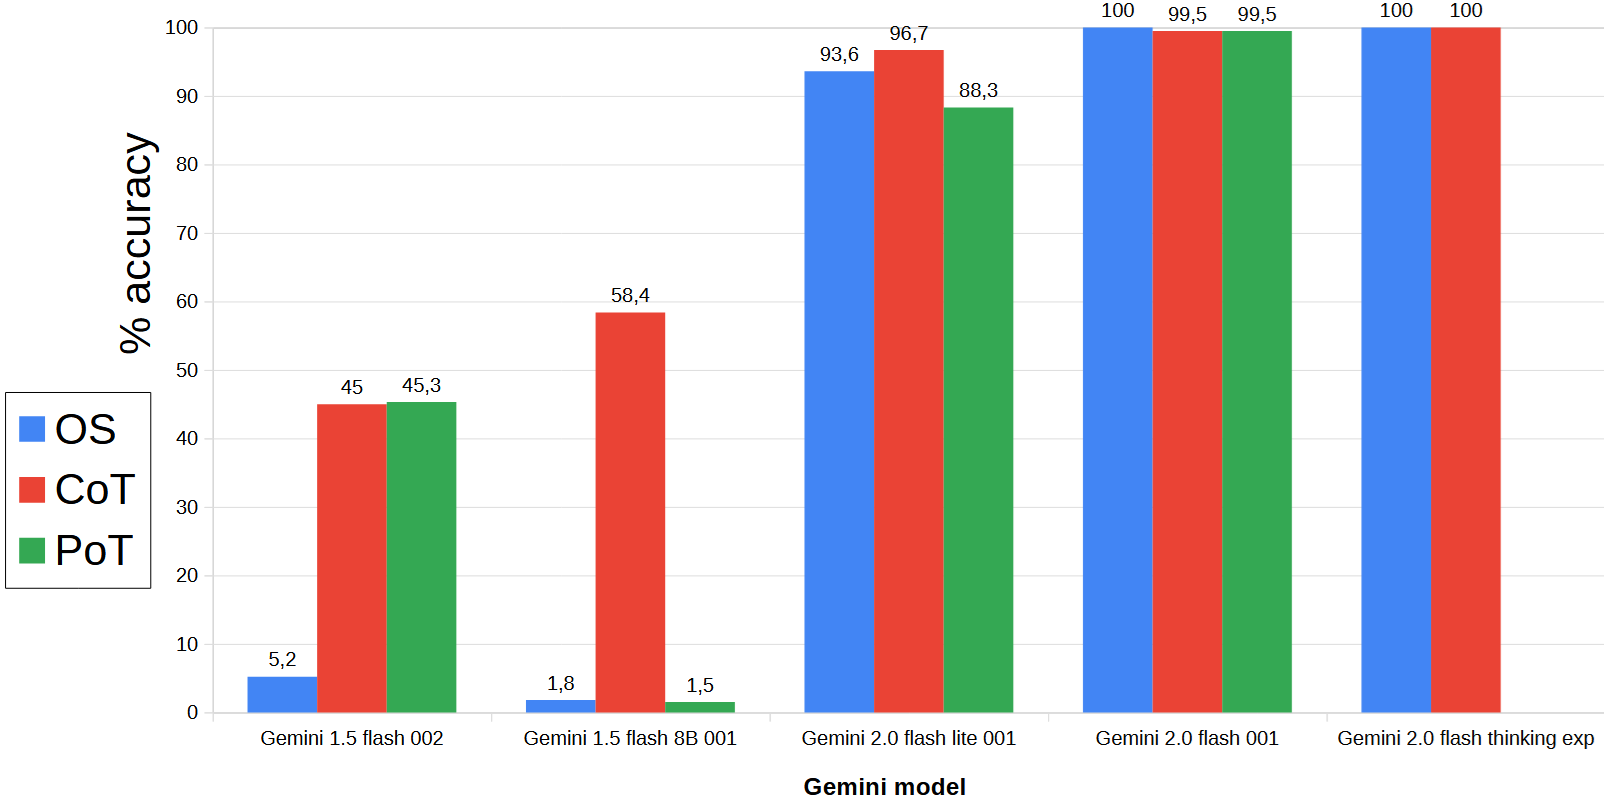
\includegraphics[width=1\textwidth]{q101Gemini.png}
            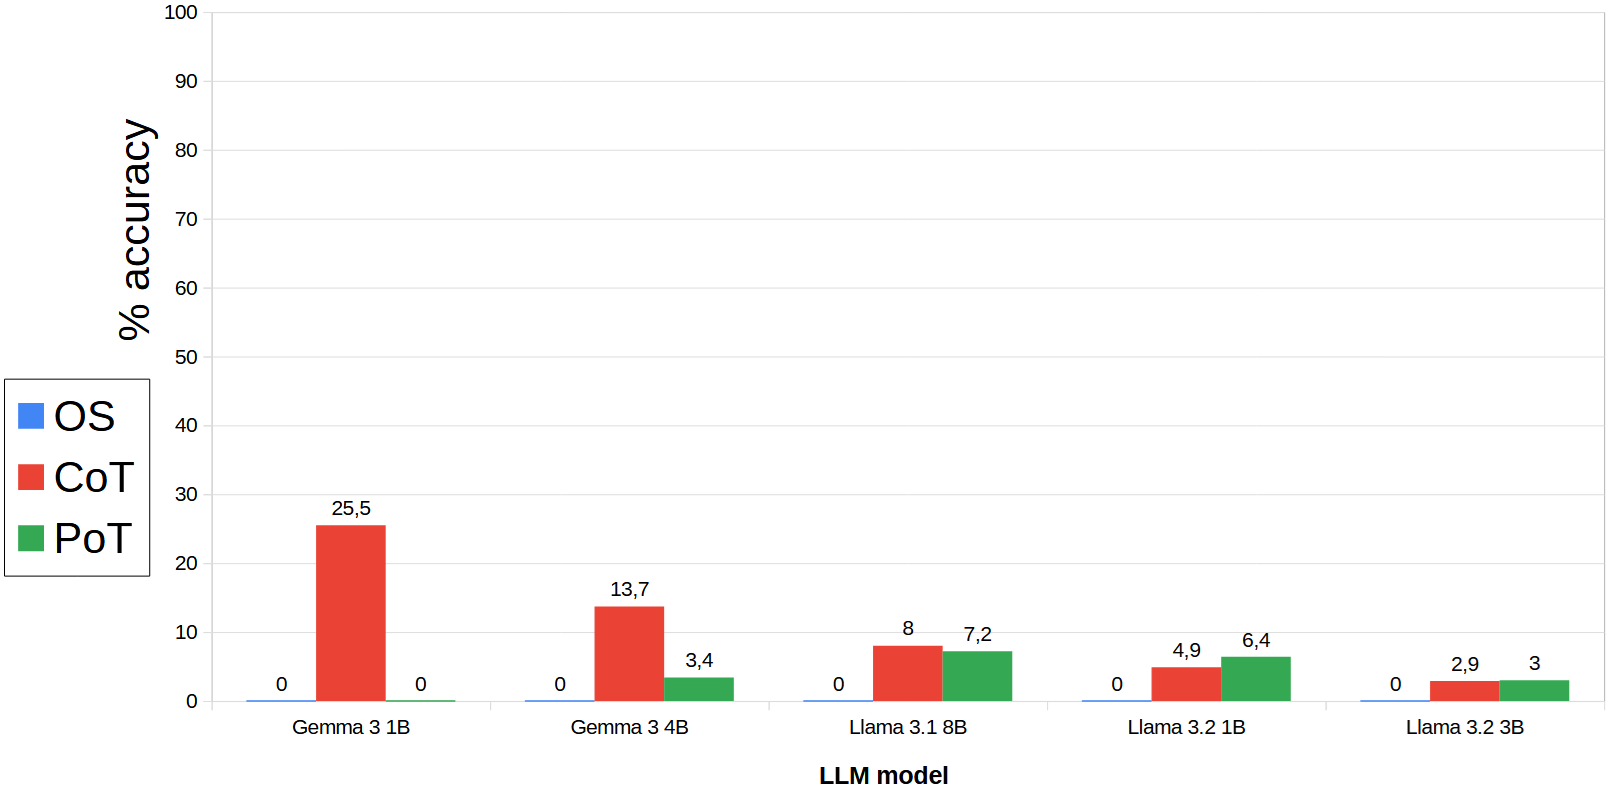
\includegraphics[width=1\textwidth]{q101Other.png}
    \caption[Accuracy on Question 1 by LLM]{Impact of prompting strategies on cumulative accuracy by large language model on question 1. Graph's data are account-level aggregation.}
    \end{figure} 
On Gemini models, a clear improvement in results can be seen as versions progress, but it should also be noted that this question has been tested on Gemini since before the release of the 2.0 family and is likely to have been included in the dataset for the new versions.\\
In Gemma and Llama, inconsistent results can be seen as the number of parameters improves, with a prevalence of correct answers using the CoT methodology, probably due to the simplicity of providing an intuitive answer and the difficulty of creating an effective solution algorithm.\\


\vspace{2cm}

\fbox{
    \parbox{\textwidth}{
    What is the maximum point in the interval x = 0 and x = pi of the function y = x*sin(x) ?
    }
}

\begin{figure}[H]
    \centering
            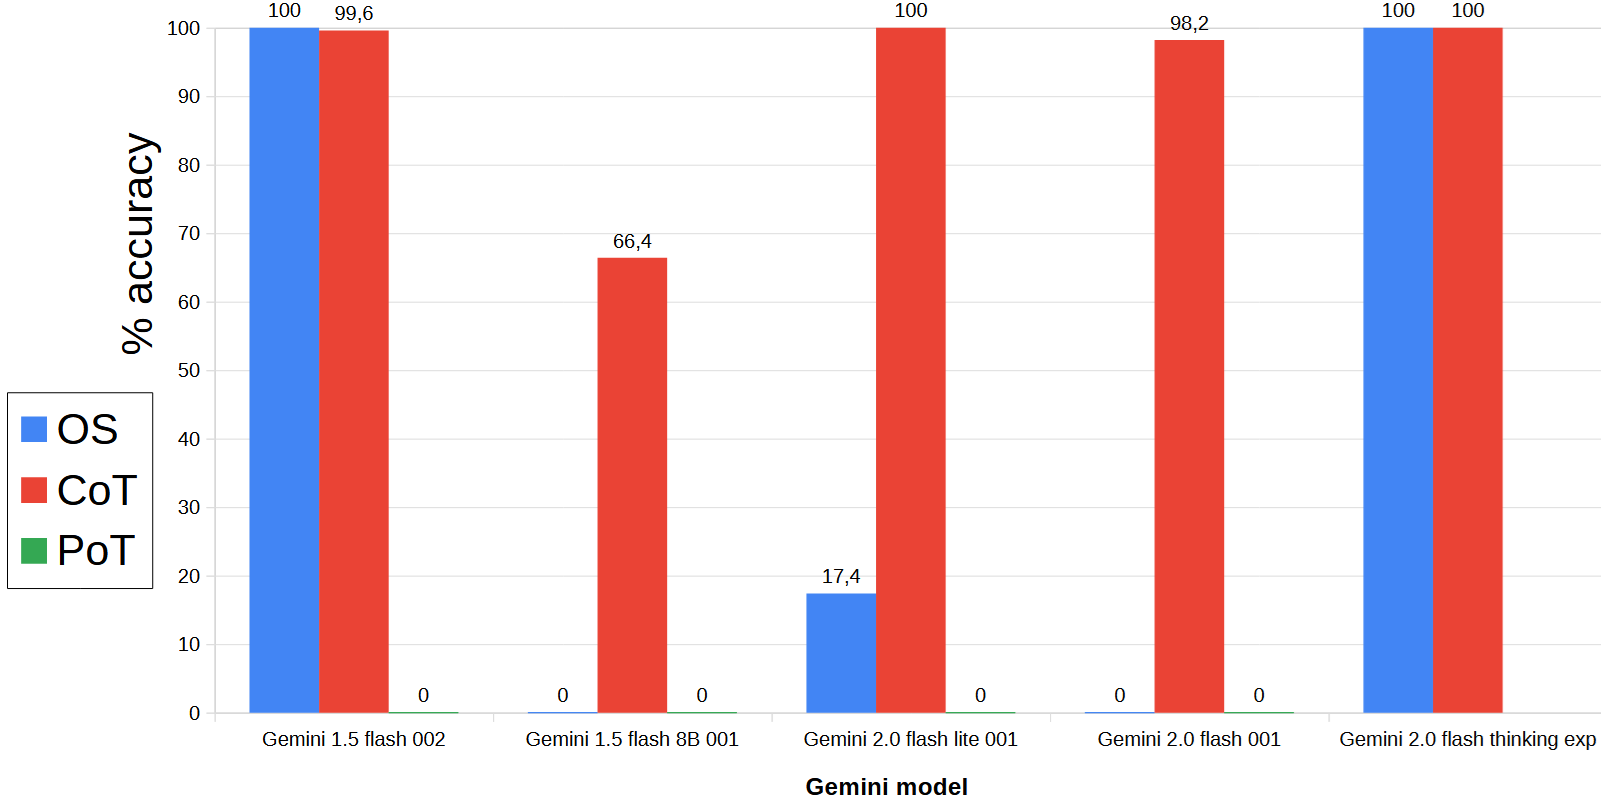
\includegraphics[width=1\textwidth]{q104Gemini.png}
            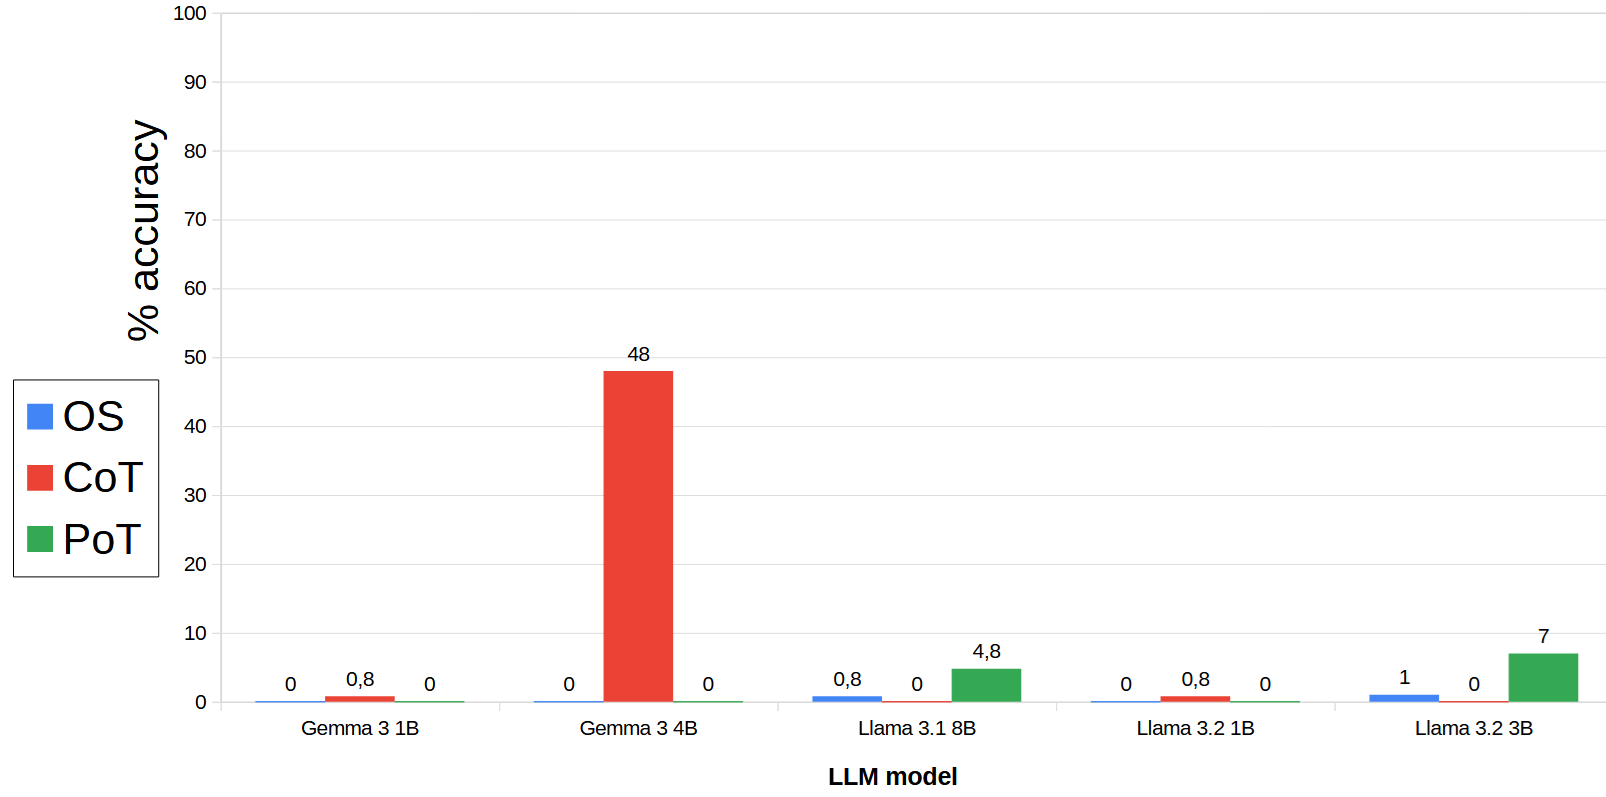
\includegraphics[width=1\textwidth]{q104Other.png}
    \caption[Accuracy on Question 2 by LLM]{Impact of prompting strategies on cumulative accuracy by large language model on question 2. Graph's data are account-level aggregation.}
    \label{fig:27}
    \end{figure} 
Good results can be seen with the CoT methodology and sometimes with OS on the Gemini and Gemma models; it is likely that the solution can be found directly in the dataset.\\
It is almost impossible to produce a working algorithm with the PoT methodology in all models.\\

\vspace{2cm}

\fbox{
    \parbox{\textwidth}{
    In a population, births are decreasing by 30 000 per year while annual deaths are stable at 350 000. The current population is 60 000 000 and the number of current births 350 000. How many years are required for the population to halve assuming stability in trends?
    }
}

\begin{figure}[H]
    \centering
            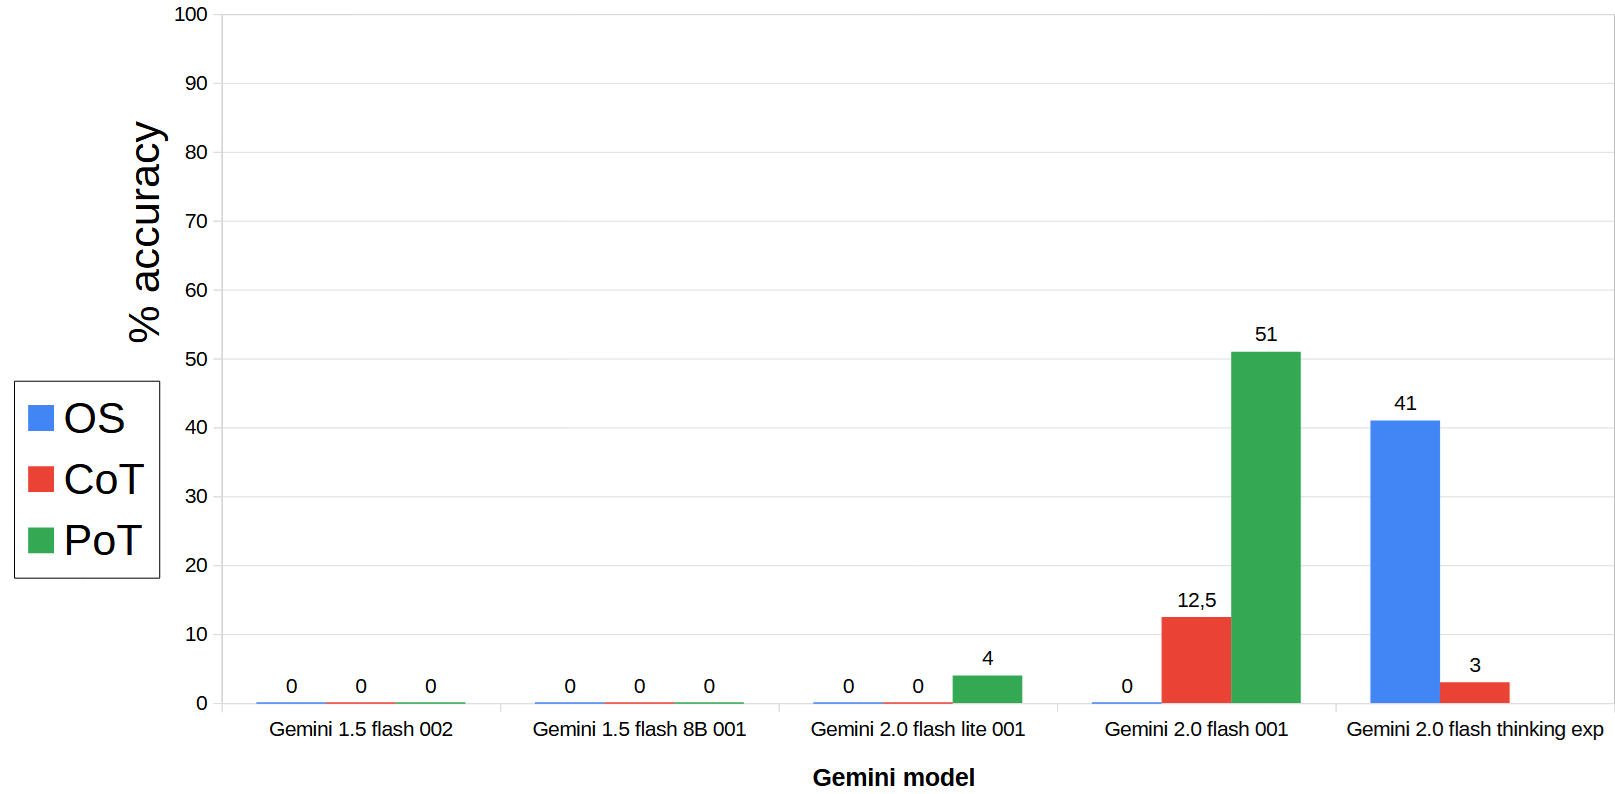
\includegraphics[width=1\textwidth]{q105Gemini.png}
            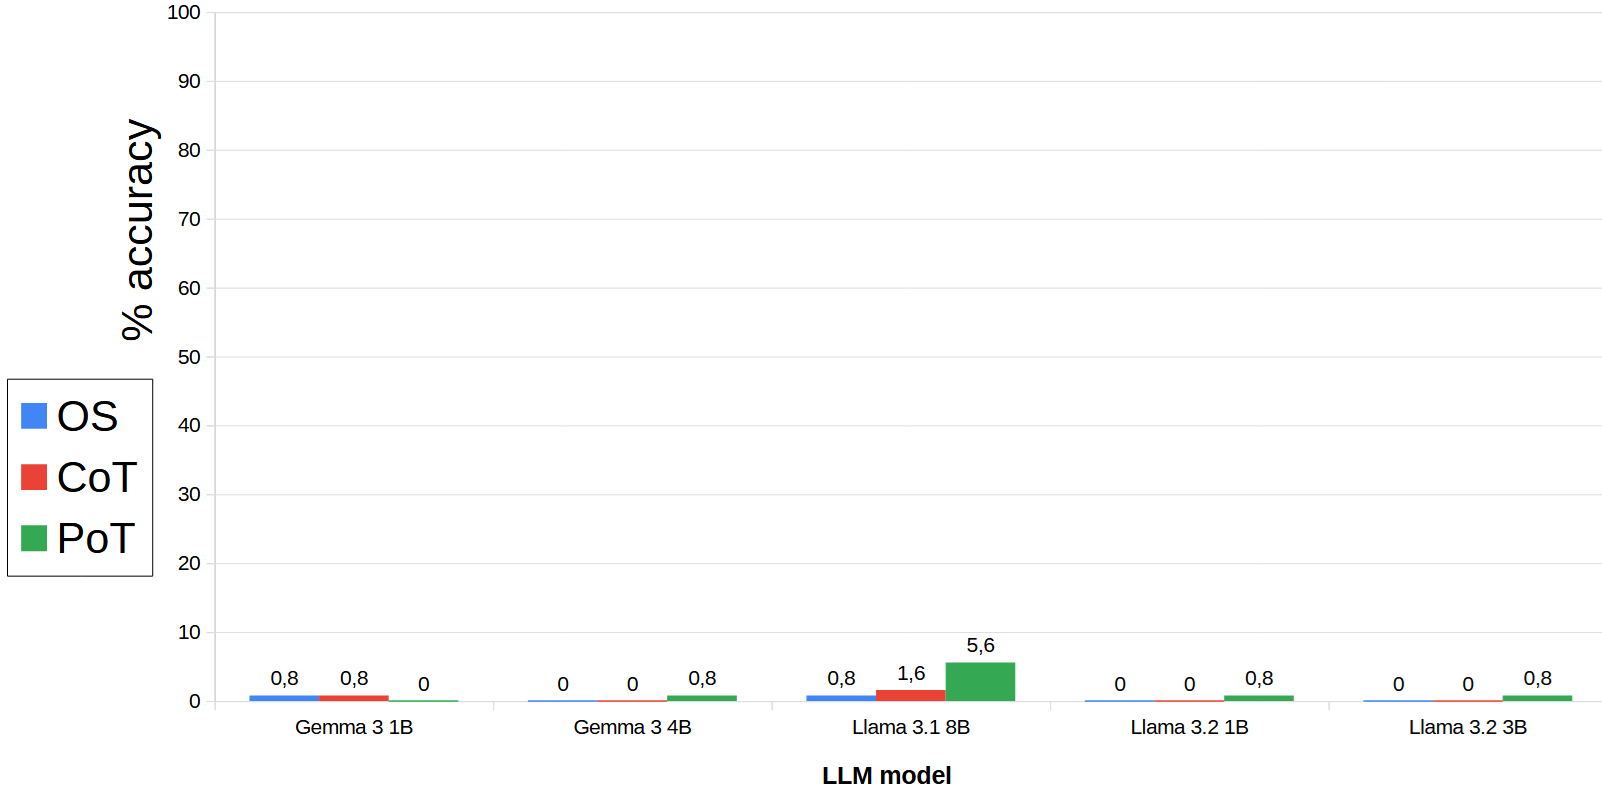
\includegraphics[width=1\textwidth]{q105Other.png}
    \caption[Accuracy on Question 3 by LLM]{Impact of prompting strategies on cumulative accuracy by large language model on question 3. Graph's data are account-level aggregation.}
    \end{figure} 
The problem is quite complex and only produces good results with PoT in Gemini 2.0 flash.\\ 
The good results obtained with OS in Gemini 2.0 flash thinking exp are probably random, given the results obtained with CoT in the same model.\\

\vspace{2cm}

\subsubsection{Common Math Problems} %102, 103
The following problems are classic and can be solved by simply applying a formula.\\
Here are the two questions in this category:\\

\fbox{
    \parbox{\textwidth}{
    A 25-year-old person invests money with an annual interest rate of 5\%. How much must he invest now to have \$1 million when he retires at age 65?
    }
}

\begin{figure}[H]
    \centering
            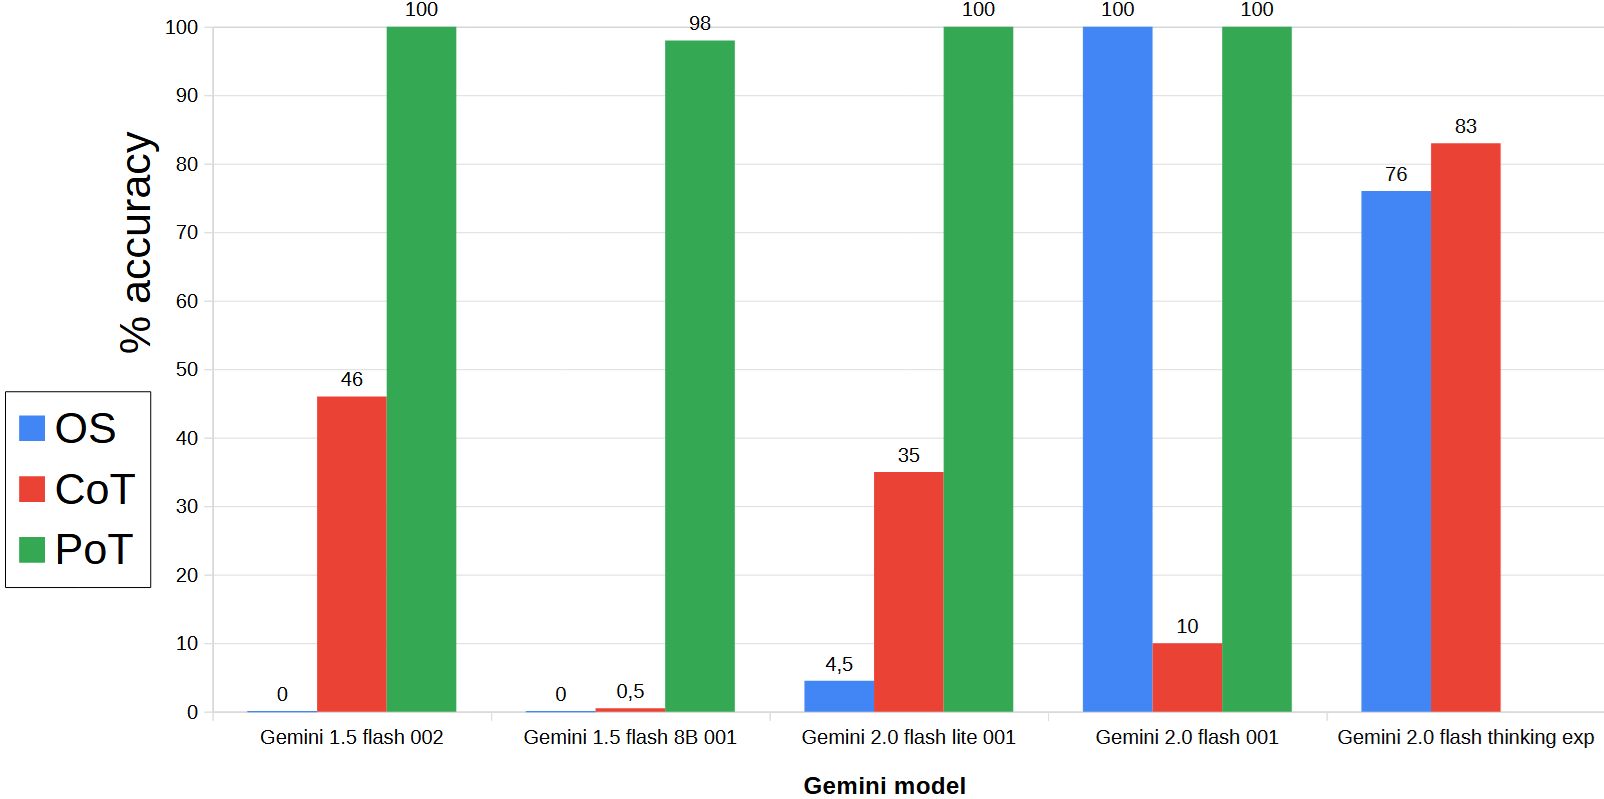
\includegraphics[width=1\textwidth]{q102Gemini.png}
            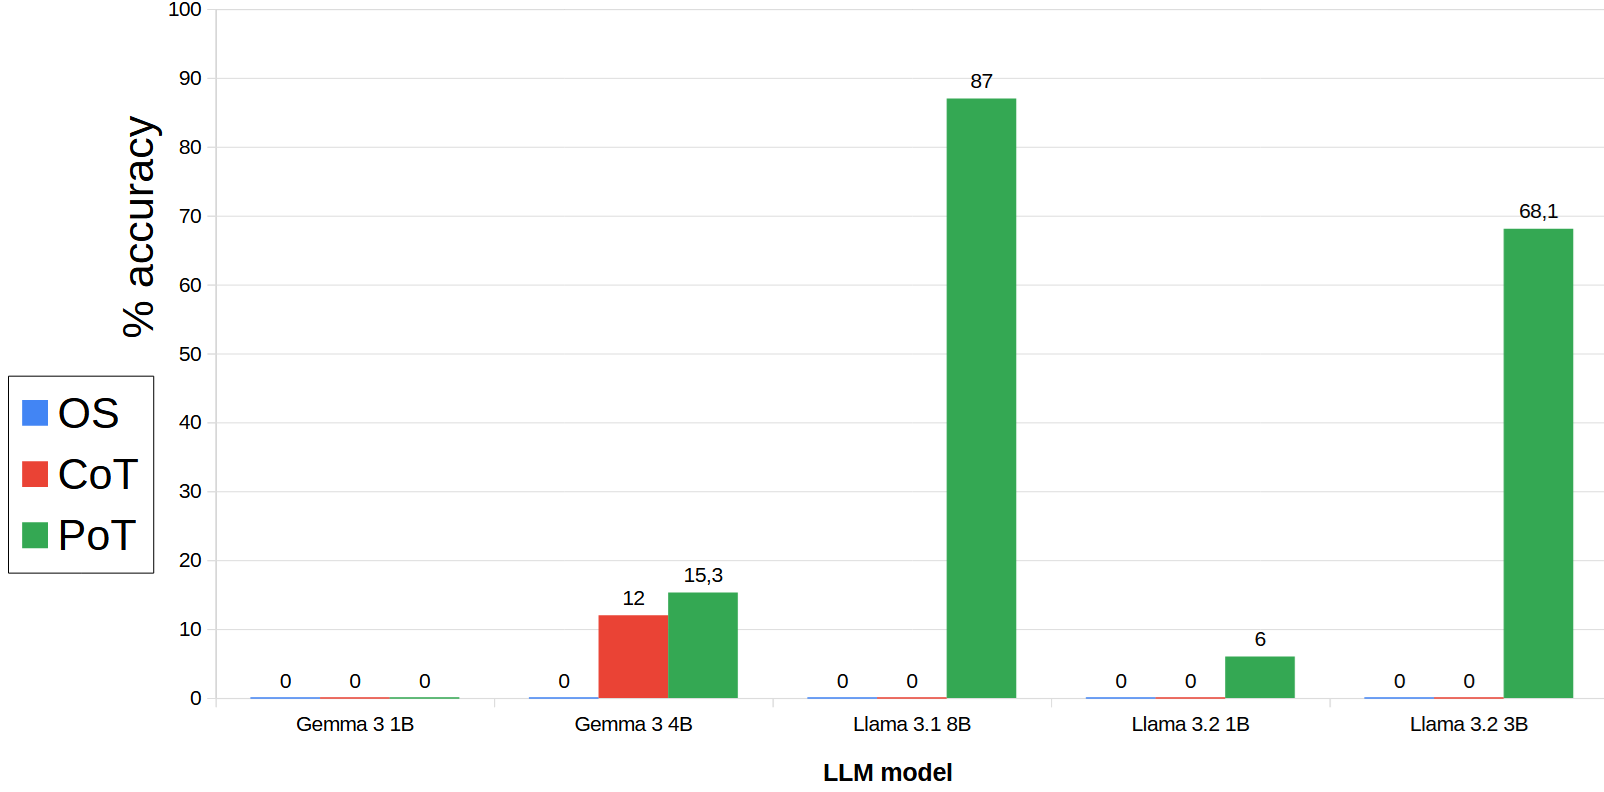
\includegraphics[width=1\textwidth]{q102Other.png}
    \caption[Accuracy on Question 4 by LLM]{Impact of prompting strategies on cumulative accuracy by large language model on question 4. Graph's data are account-level aggregation.}
    \end{figure} 
The results are excellent when using PoT with Gemini and with open models with a sufficient number of parameters.\\

\vspace{2cm}

\fbox{
    \parbox{\textwidth}{
    A 25-year-old person invests money with an annual interest of 6 compounded continuously. How much must he invest now to have \$1 million when he retires at age 65?
    }
}

\begin{figure}[H]
    \centering
            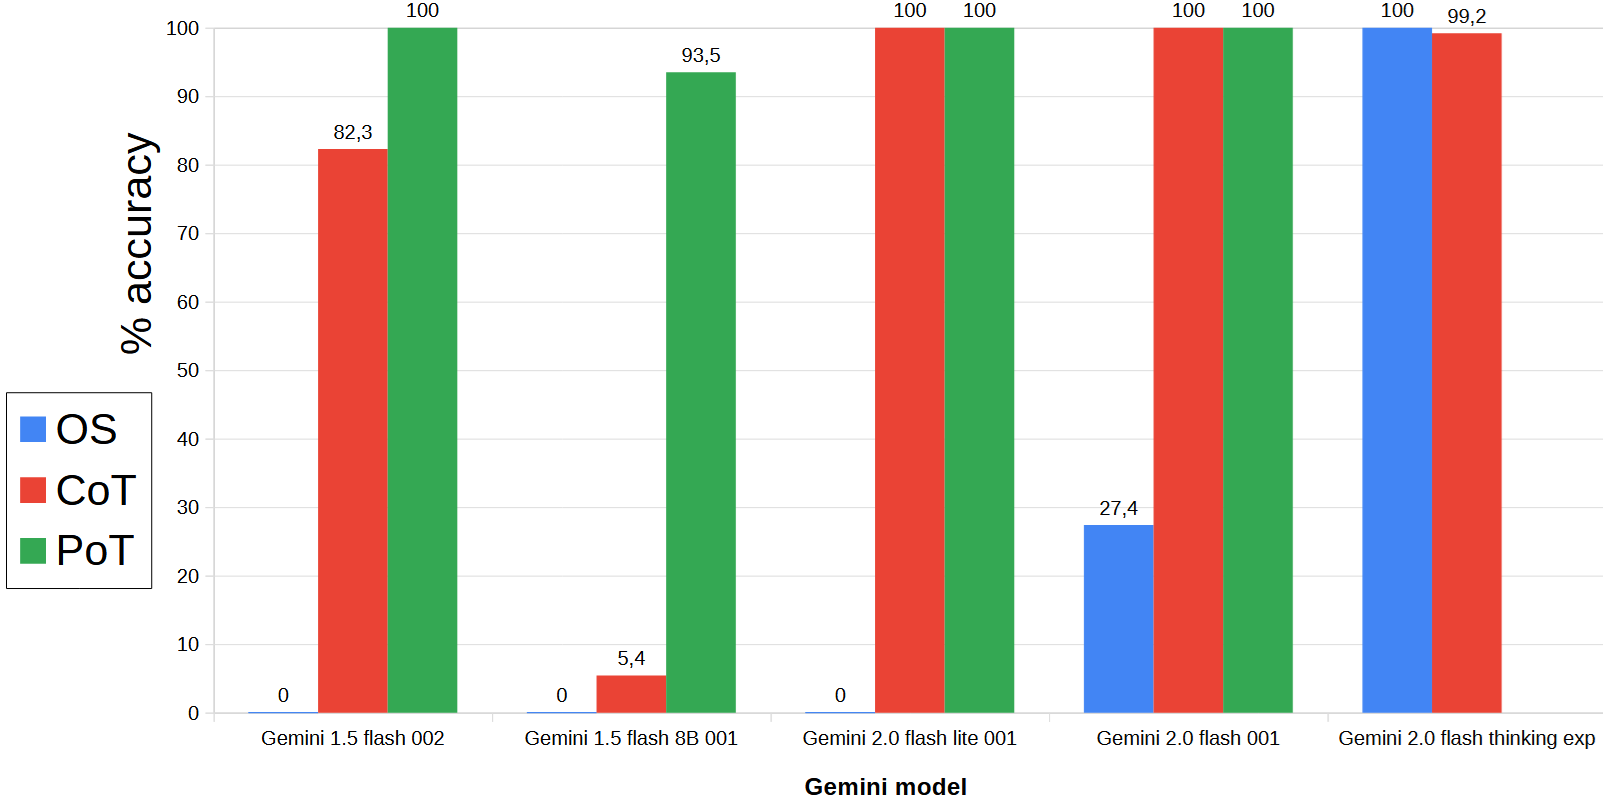
\includegraphics[width=1\textwidth]{q103Gemini.png}
            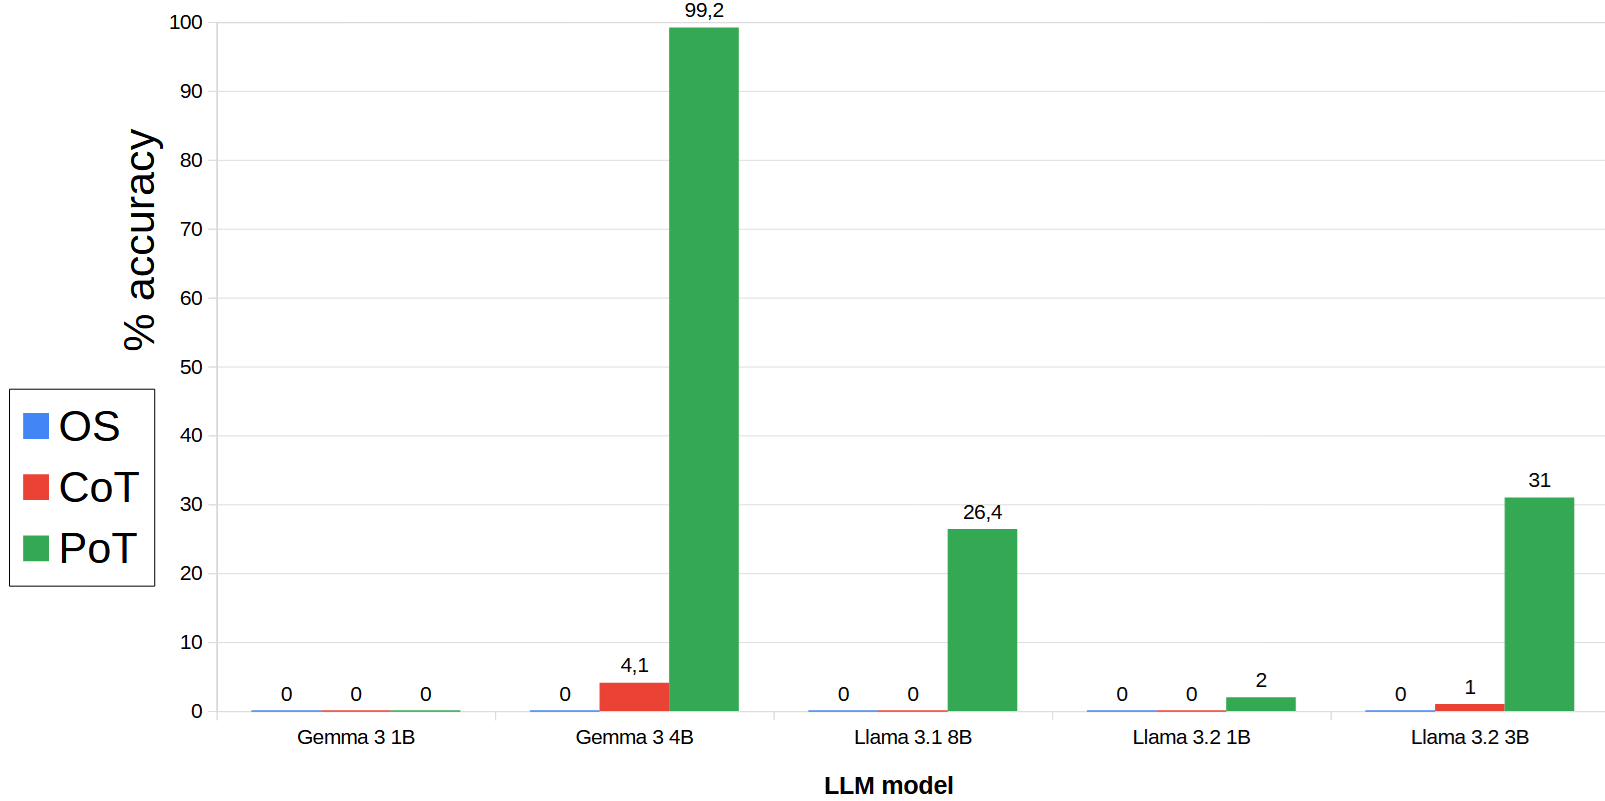
\includegraphics[width=1\textwidth]{q103Other.png}
    \caption[Accuracy on Question 5 by LLM]{Impact of prompting strategies on cumulative accuracy by large language model on question 5. Graph's data are account-level aggregation.}
    \end{figure} 
As with the previous question, the results are excellent when using PoT with Gemini and with open models with a sufficient number of parameters.\\

\vspace{2cm}
\subsubsection{Sudoku} %106
\fbox{
    \parbox{\textwidth}{
    Solve the sudoku in the image.
    
     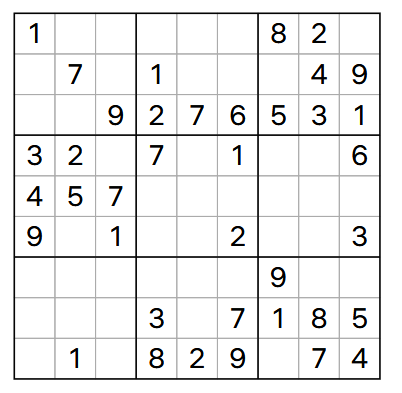
\includegraphics[width=1\textwidth]{img106.png}
    }
}

\begin{figure}[H]
    \centering
            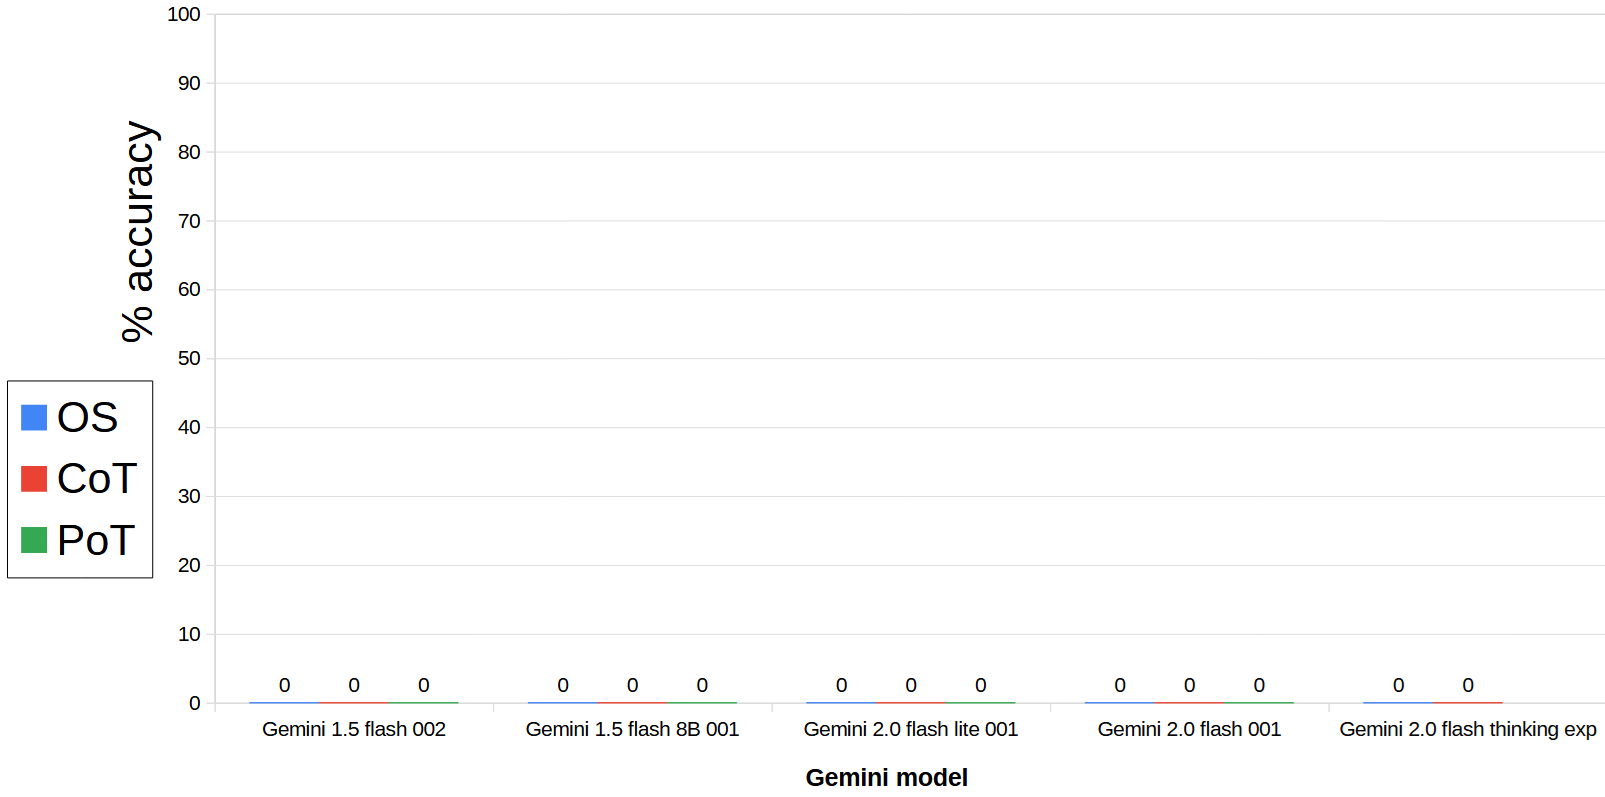
\includegraphics[width=1\textwidth]{q106Gemini.png}
    \caption[Accuracy on Question 6 by LLM]{Impact of prompting strategies on cumulative accuracy by large language model on question 6. Graph's data are account-level aggregation.}
    \end{figure} 
Gemini does not seem capable of solving Sudoku, even though it provides a partially coherent, invented answer each time.\\
Open models were not used with images for technical simplicity.\\

\vspace{2cm}
\subsection{Factuality}
The questions in this category were resolved using the OS methodology, except for the first one, for which CoT was also used.\\
Data relating to Gemini 2.0 flash thinking exp is only available for certain questions due to a speed limit restriction for free accounts introduced during the testing phase.\\
\subsubsection{Factual Pitfalls} %201, 202, 203, 204
This category contains some complex questions that aim to verify the accuracy of details and adherence to reality.\\

\fbox{
    \parbox{\textwidth}{
    How many subsections of Article 140 of the Italian Constitution are there?
    }
}

\begin{figure}[H]
    \centering
            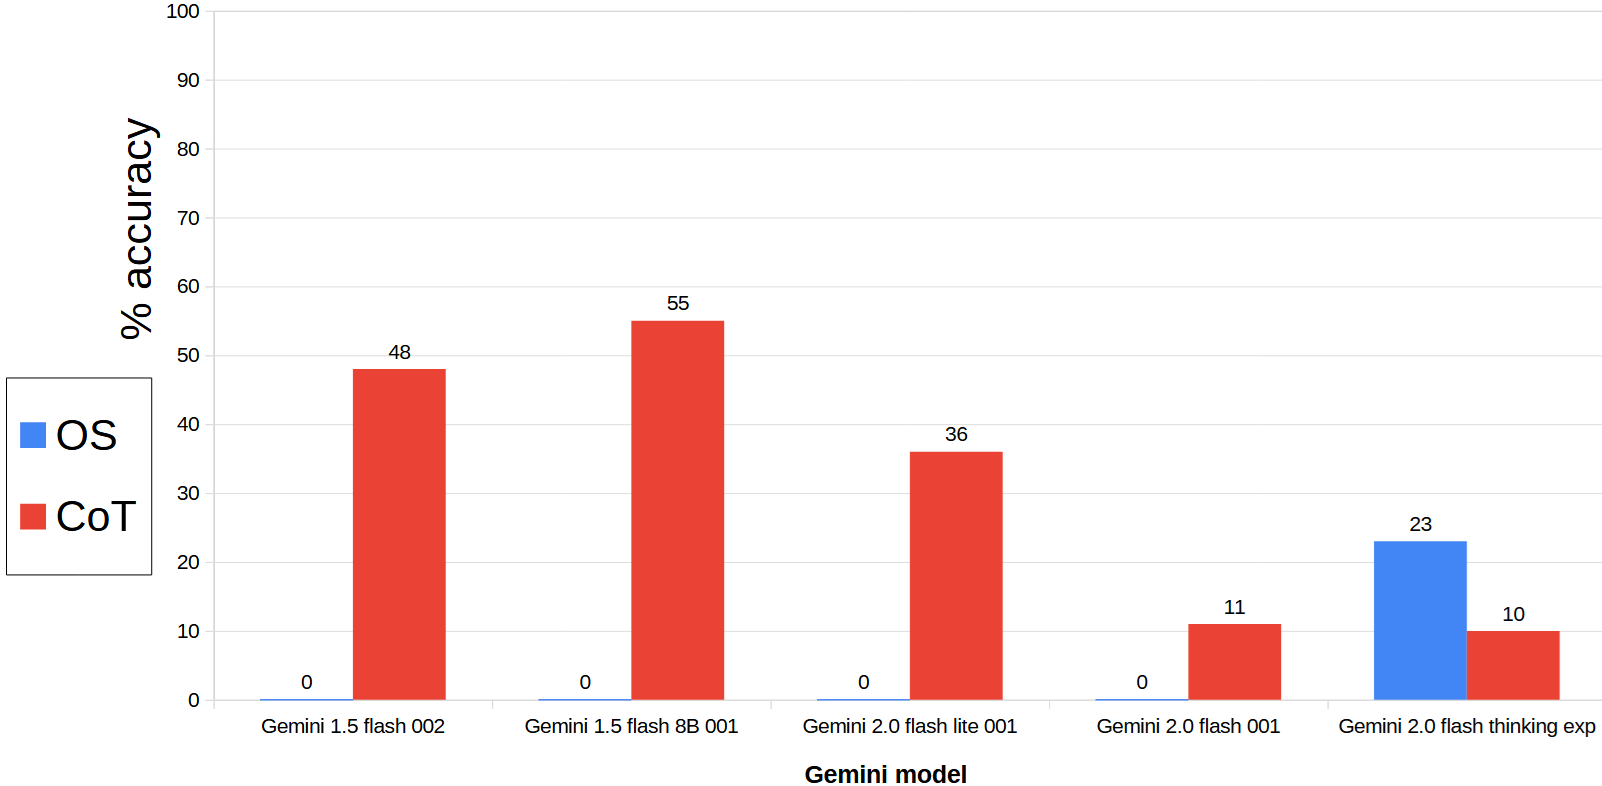
\includegraphics[width=1\textwidth]{q201Gemini.png}
            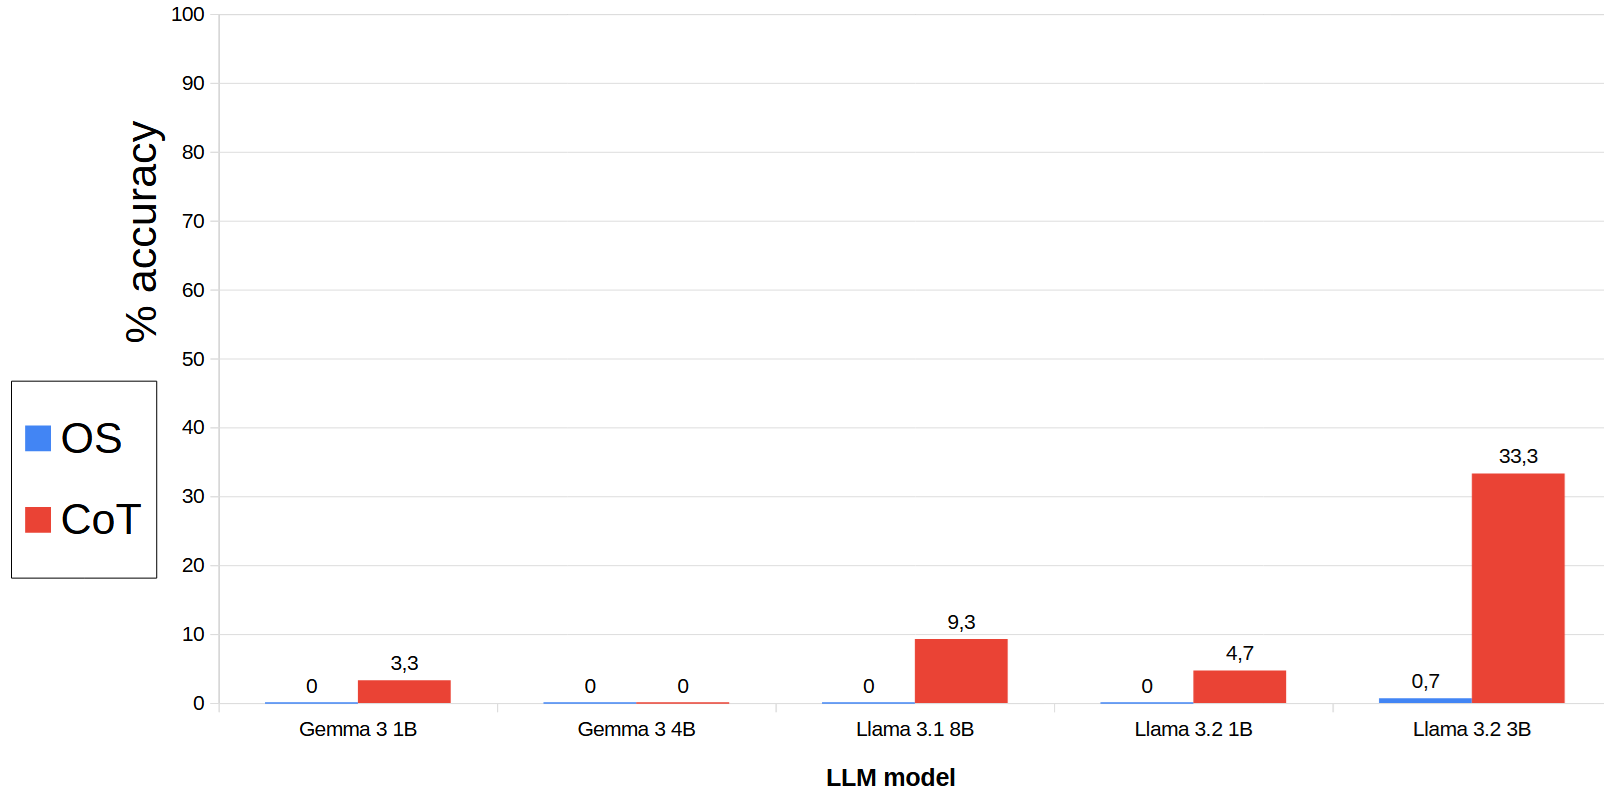
\includegraphics[width=1\textwidth]{q201Other.png}
    \caption[Accuracy on Question 7 by LLM]{Impact of prompting strategies on cumulative accuracy by large language model on question 7. Graph's data are account-level aggregation.}
    \label{fig:32}
    \end{figure} 
A trick question that yields acceptable results, especially when using the CoT methodology.\\

\vspace{2cm}

\fbox{
    \parbox{\textwidth}{
    How many months did it take Salvini to get a bachelor degree?
    }
}

\begin{figure}[H]
    \centering
            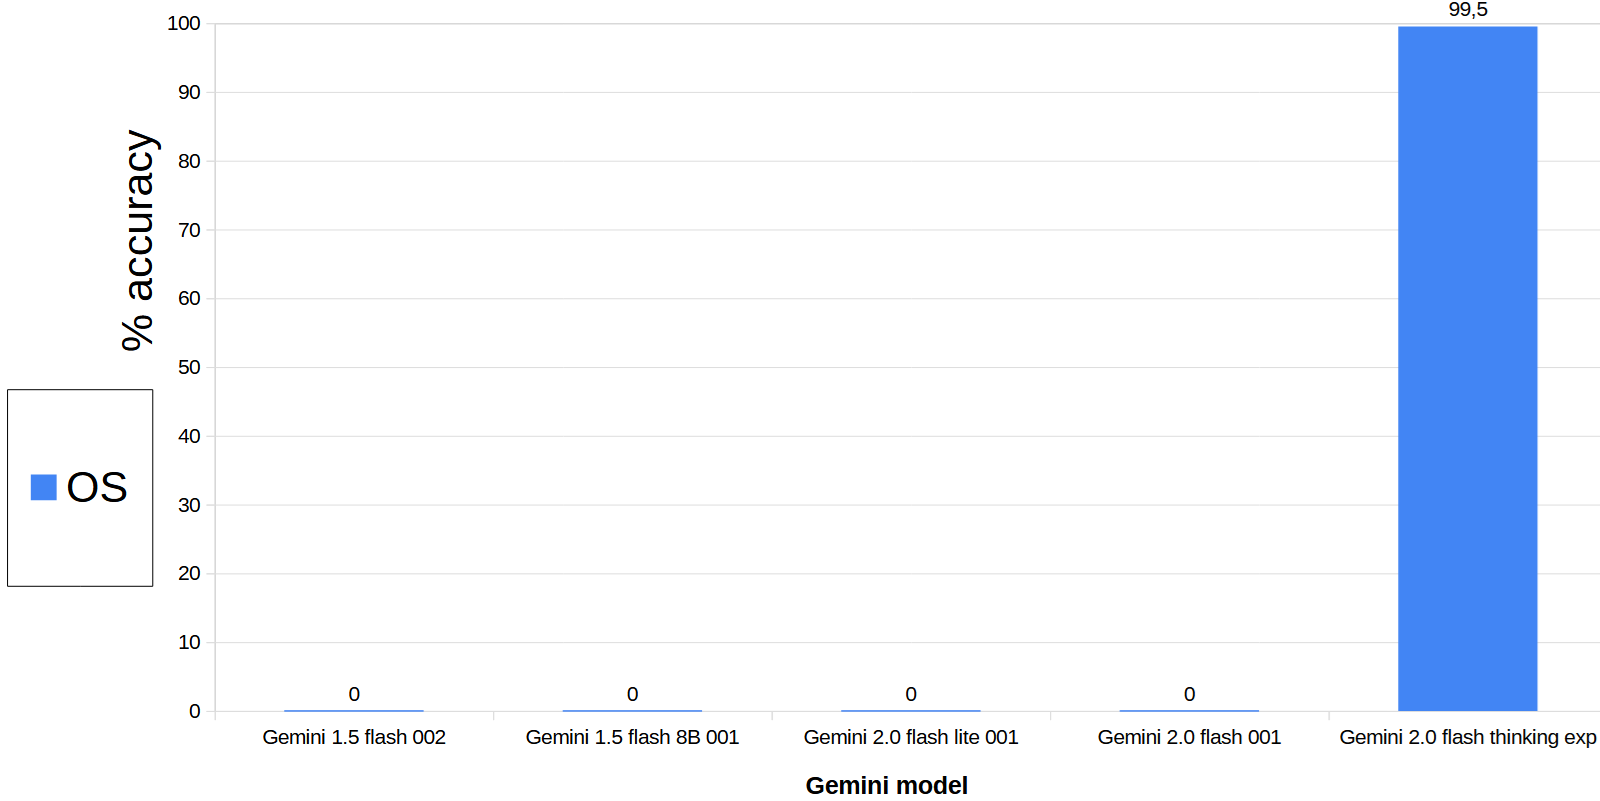
\includegraphics[width=1\textwidth]{q202Gemini.png}
            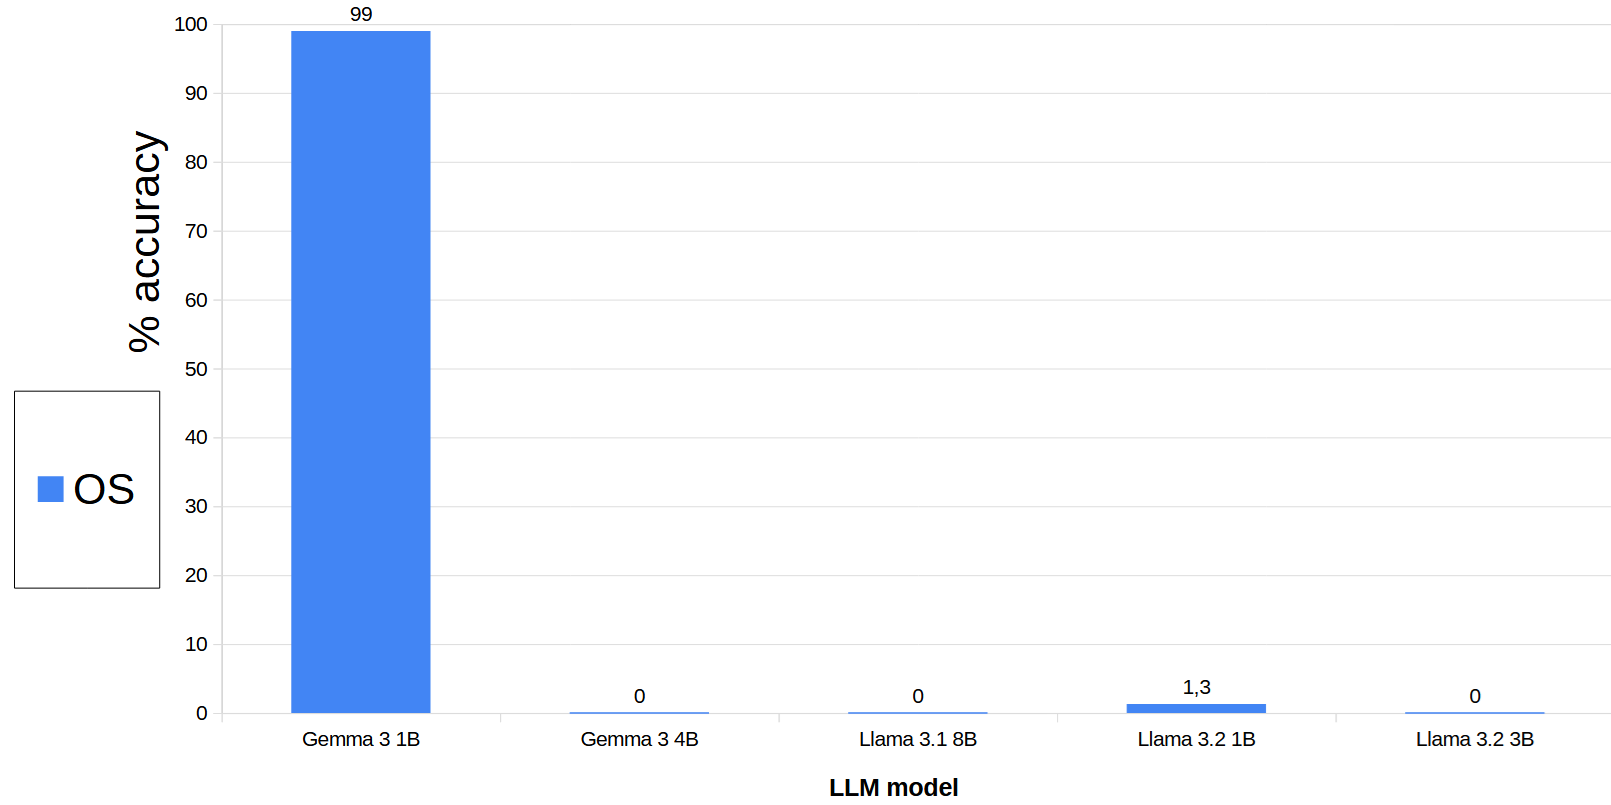
\includegraphics[width=1\textwidth]{q202Other.png}
    \caption[Accuracy on Question 8 by LLM]{Impact of prompting strategies on cumulative accuracy by large language model on question 8. Graph's data are account-level aggregation.}
    \label{fig:33}
    \end{figure} 
The results are inconsistent; it is likely that there is an overestimation of correct responses caused by considering the model to be right when it does not know or refuses to respond.\\

\vspace{2cm}

\fbox{
    \parbox{\textwidth}{
    What is the sum of the different colors and columns in the flag of Moldova?
    }
}

\begin{figure}[H]
    \centering
            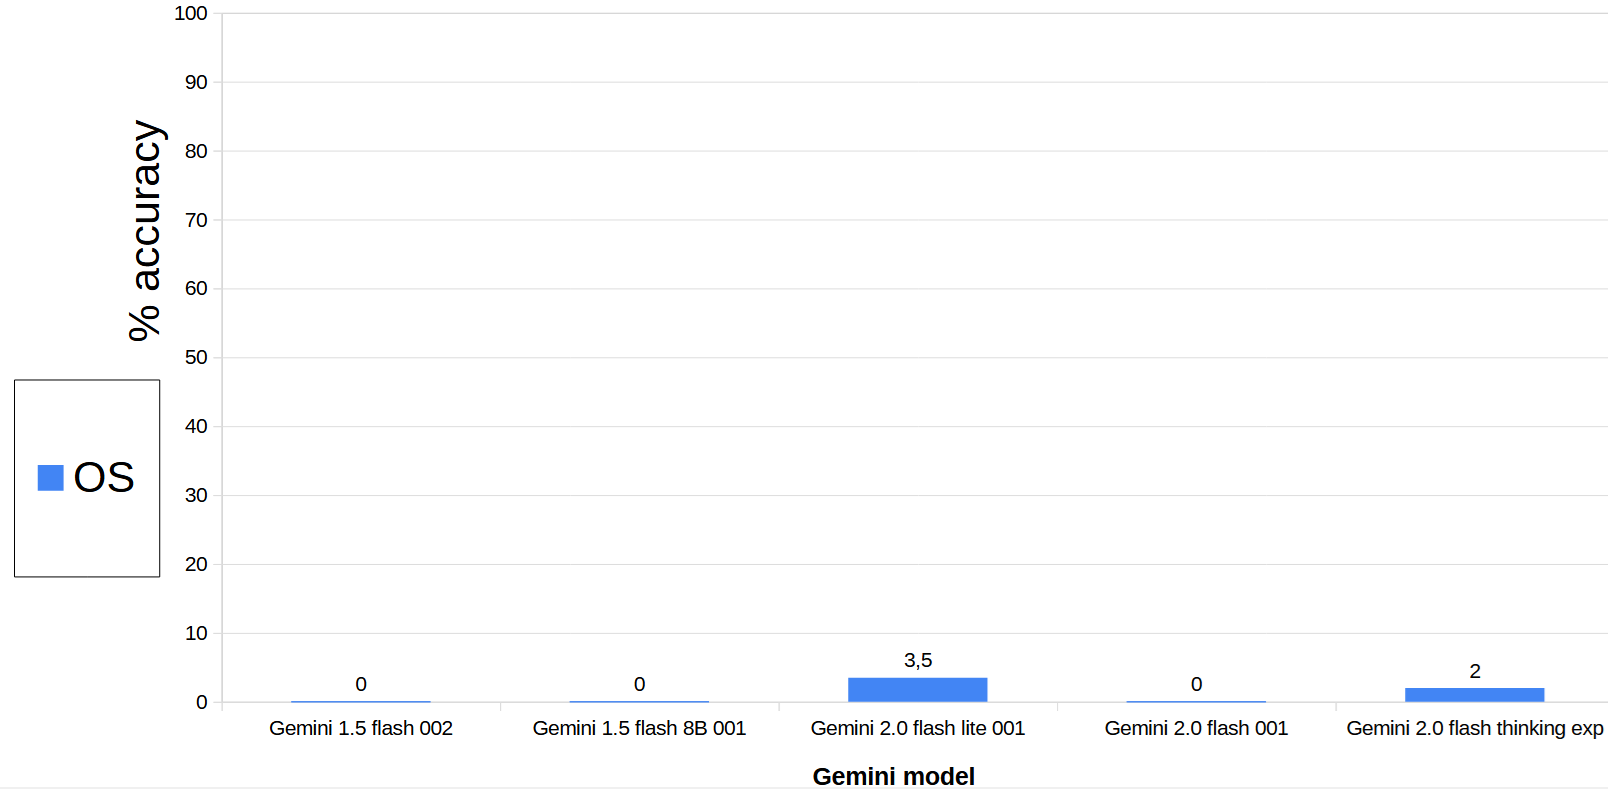
\includegraphics[width=1\textwidth]{q203Gemini.png}
            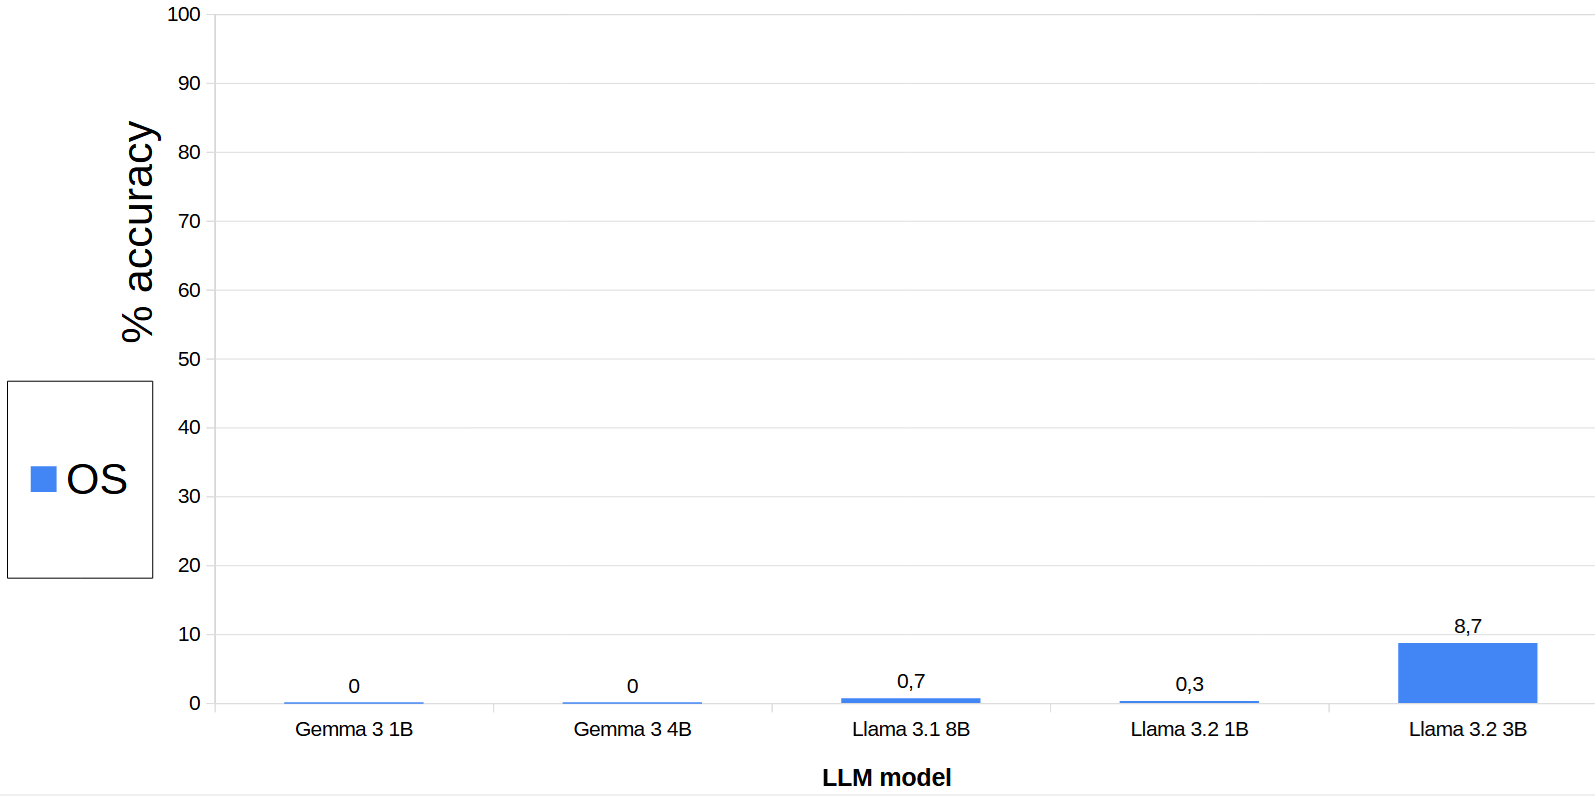
\includegraphics[width=1\textwidth]{q203Other.png}
    \caption[Accuracy on Question 9 by LLM]{Impact of prompting strategies on cumulative accuracy by large language model on question 9. Graph's data are account-level aggregation.}
    \end{figure} 
All models show difficulty interpreting flags with complex sections.\\

\vspace{2cm}

\fbox{
    \parbox{\textwidth}{
    Sum the number of horizontal stripes and the number of different colors in the flag of Mozambique.
    }
}

\begin{figure}[H]
    \centering
            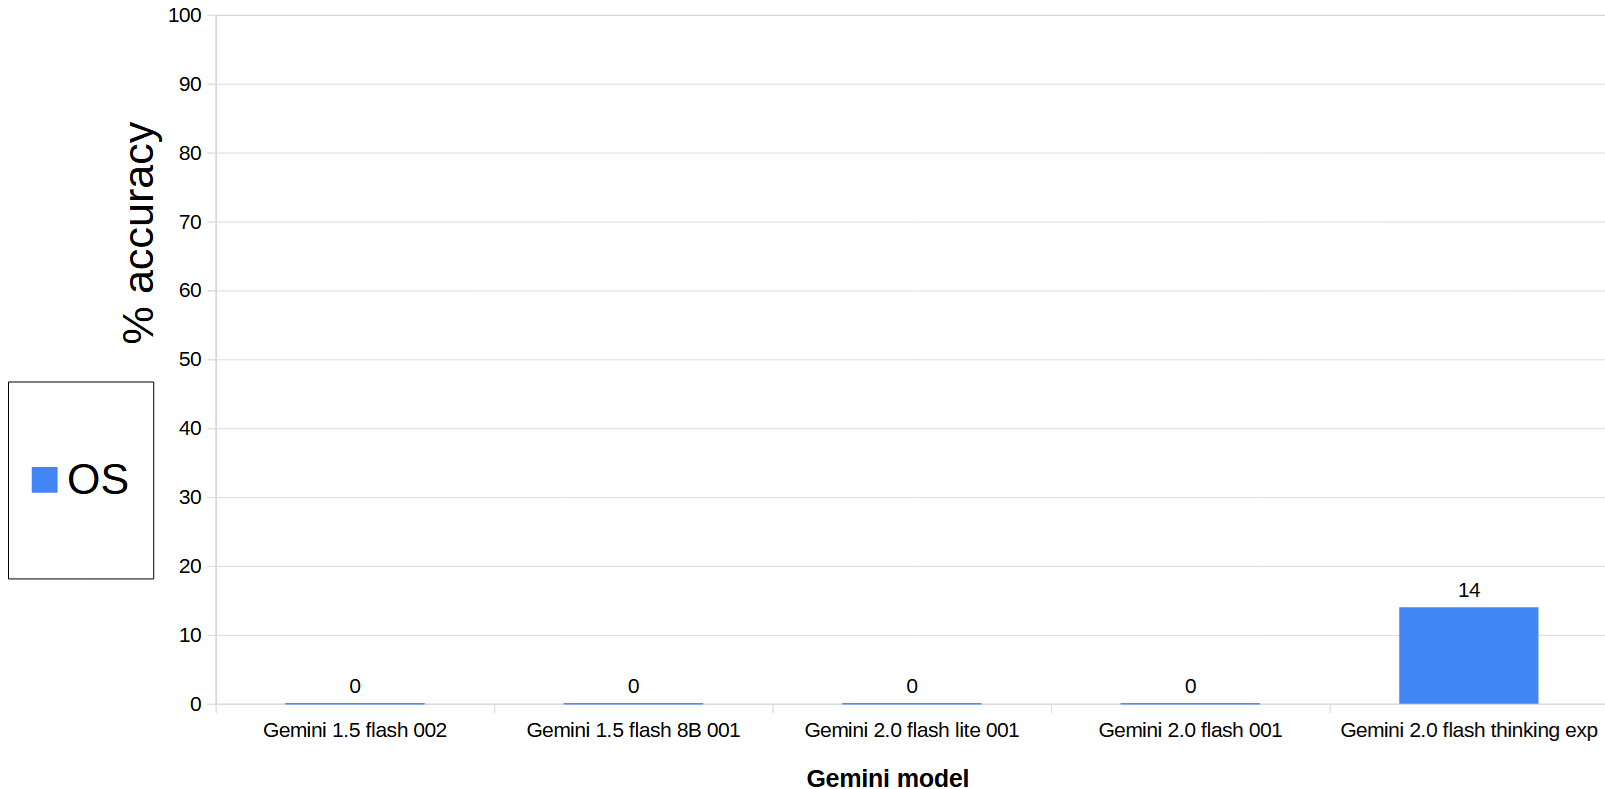
\includegraphics[width=1\textwidth]{q204Gemini.png}
            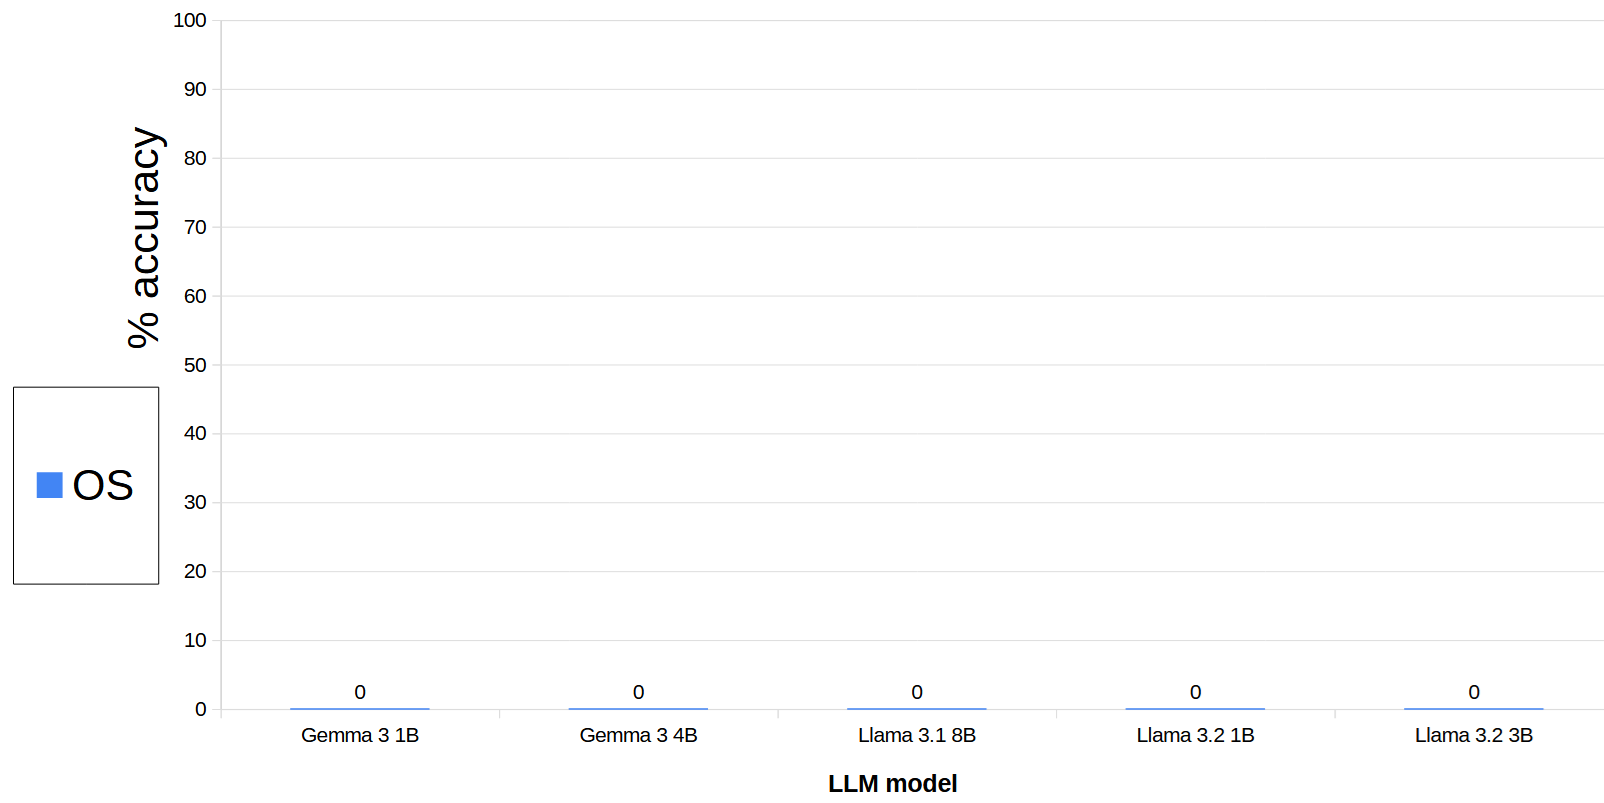
\includegraphics[width=1\textwidth]{q204Other.png}
    \caption[Accuracy on Question 10 by LLM]{Impact of prompting strategies on cumulative accuracy by large language model on question 10. Graph's data are account-level aggregation.}
    \end{figure} 
As in the previous question, the models show difficulty interpreting flags with complex sections.\\

\vspace{2cm}
\subsubsection{Russell's theory of descriptions} %205, 206
In questions in thi
s category, the correct answer is the third option, as the assumption is incorrect.\\

\fbox{
    \parbox{\textwidth}{
    The current king of France is dead.\\
Evaluate whether this statement is:\\
1- True
2- false
3- other
    }
}

\begin{figure}[H]
    \centering
            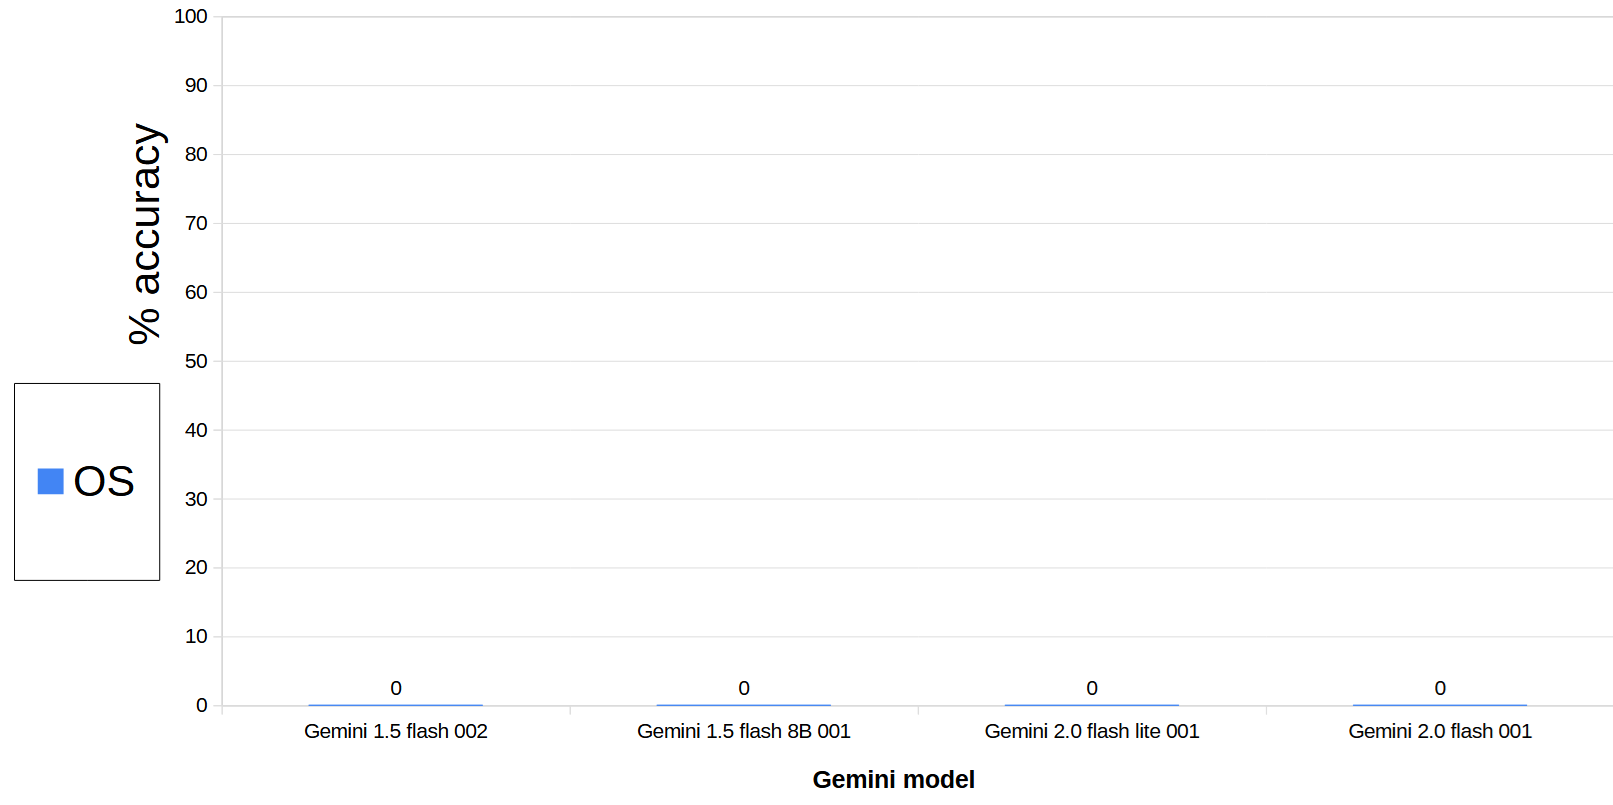
\includegraphics[width=1\textwidth]{q205Gemini.png}
            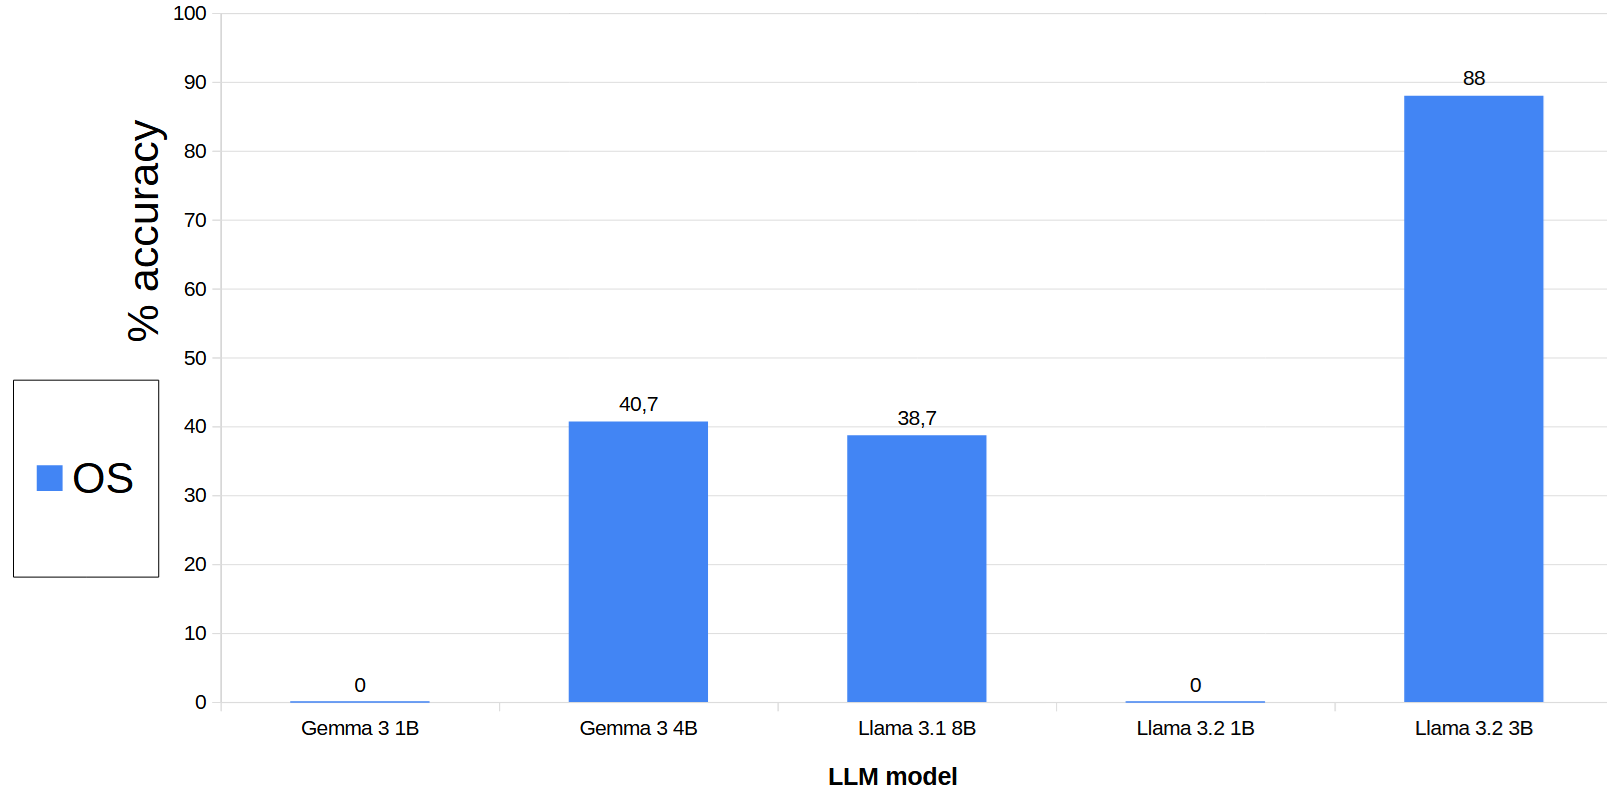
\includegraphics[width=1\textwidth]{q205Other.png}
    \caption[Accuracy on Question 11 by LLM]{Impact of prompting strategies on cumulative accuracy by large language model on question 11. Graph's data are account-level aggregation.}
    \end{figure} 
Despite all of Gemini's incorrect answers, the open models achieve good results.\\

\vspace{2cm}

\fbox{
    \parbox{\textwidth}{
    I find it pleasant to yawn as soon as I am awake, while yawning as soon as I am asleep does not appeal to me.\\
Assuming that the interlocutor is not lying, the following statement is to be considered:\\
1-True
2-false
3-other
    }
}

\begin{figure}[H]
    \centering
            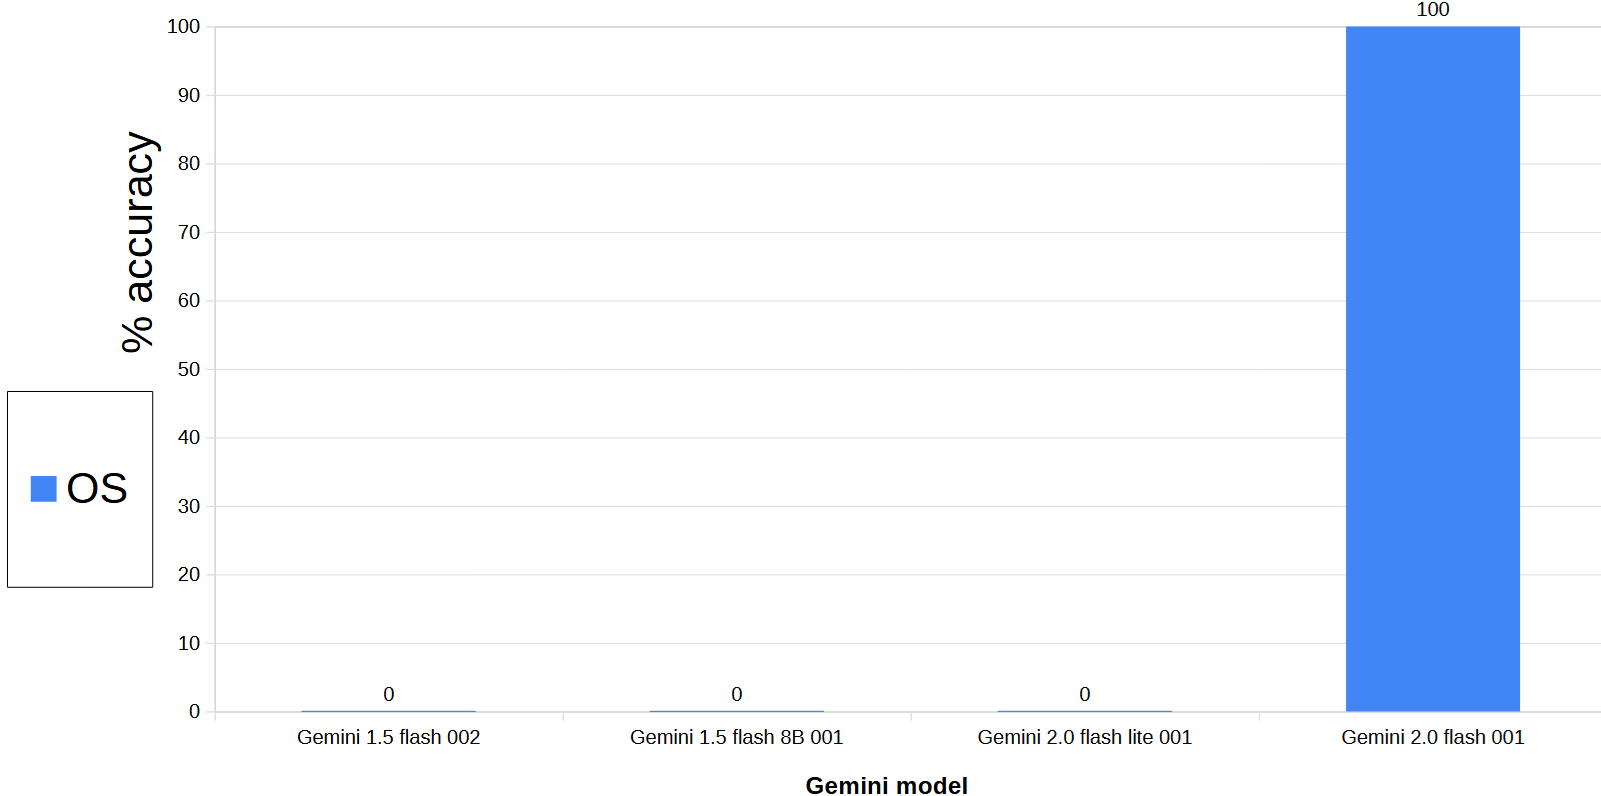
\includegraphics[width=1\textwidth]{q206Gemini.png}
            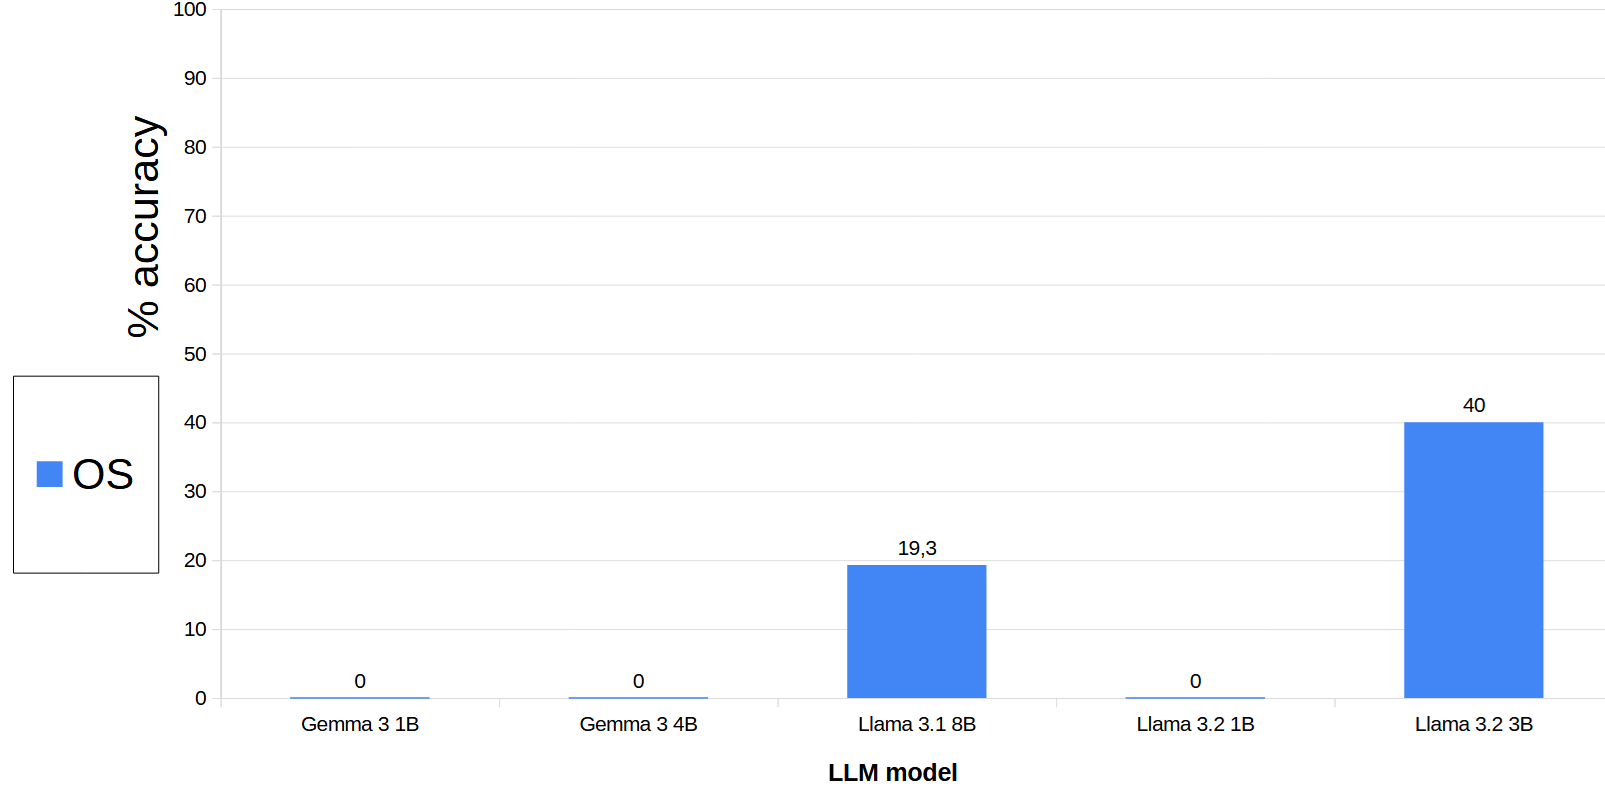
\includegraphics[width=1\textwidth]{q206Other.png}
    \caption[Accuracy on Question 12 by LLM]{Impact of prompting strategies on cumulative accuracy by large language model on question 12. Graph's data are account-level aggregation.}
    \end{figure} 
Very similar to the previous question, but with the total accuracy of the latest Gemini model taken into account.\\

\vspace{2cm}

\subsection{Sequential Problem Solving}
This category contains a total of 10 questions and shows how LLMs struggle to plan when faced with overlapping plans.\\
Open LLMs and the Gemini 1.5 family did not achieve significant results, having an accuracy close to zero.\\

\subsubsection{Wolf, Goat and Cabbage} %301, 302
\fbox{
    \parbox{\textwidth}{
   A farmer must carry a cabbage, a goat and a wolf across the river. The farmer can carry only himself or himself together with only one of the other 3 at a time.
The cabbage, the goat and the wolf cannot cross the river without the farmer.
The cabbage and the goat cannot stay on the same bank in the absence of the farmer.
The goat and the wolf cannot stay on the same bank in the absence of the farmer.
    }
}

\begin{figure}[H]
    \centering
            \includegraphics[width=1\textwidth]{q301Gemini.png}
            \includegraphics[width=1\textwidth]{q301Other.png}
    \caption[Accuracy on Question 13 by LLM]{Impact of prompting strategies on cumulative accuracy by large language model on question 13. Graph's data are account-level aggregation.}
    \label{fig:38}
    \end{figure} 
The Gemini 2.0 family seems to show some interesting improvements, but as shown by the following question, when the problem is obscured, there is a complete change of pace.\\

\vspace{2cm}

\fbox{
    \parbox{\textwidth}{
Z must carry A, B and a C across two arrays, so that all three are on the second array. Z can carry only himself or himself together with only one of the other 3 at a time.
A, B and C cannot change array without Z.
A and B cannot stay on the same array in the absence of Z.
B and C cannot stay on the same array in the absence of Z.
    }
}

\begin{figure}[H]
    \centering
            \includegraphics[width=1\textwidth]{q302Gemini.png}
            \includegraphics[width=1\textwidth]{q302Other.png}
    \caption[Accuracy on Question 14 by LLM]{Impact of prompting strategies on cumulative accuracy by large language model on question 14. Graph's data are account-level aggregation.}
    \end{figure} 
The results obtained in this question show that by not allowing the model to refer back to a known problem, the quality of the proposed solution decreases significantly.\\

\vspace{2cm}

\subsubsection{Blocks World} %303, 304
In this category too, the results of the two questions asked are rather disappointing.\\
\fbox{
    \parbox{\textwidth}{
Three blocks (labeled A, B, and C) rest on a table. The blocks must be stacked such that block A is atop block B, and block B is atop block C. The problem starts with the following configuration:\\

[B], [A, C], []\\

    Block B is on the table in Stack 1 at the first position.\\
    Block C (second position in stack2) is atop block A (first position), both in Stack 2.\\
    Stack 3 is empty.\\

A valid move is popping C from Stack 2 and pushing it onto Stack 3:\\

[B], [A], [C]\\

An INVALID move would be popping A because it is not at the end of the array.\\

The goal configuration is [C, B, A] in one of the stacks, where C is at the bottom, B is in the middle, and A is on top. Blocks can only be moved one at a time, and each move follows a LIFO (Last In, First Out) policy:\\

    A push operation adds an element only at the end of the array (no insertion in the middle).\\
    A pop operation removes an element only from the end of the array.\\

Solve this problem, following the restraints and going on until the exact solution is reached or the 19th step is reached.
    }
}

\begin{figure}[H]
    \centering
            \includegraphics[width=1\textwidth]{q303Gemini.png}
            \includegraphics[width=1\textwidth]{q303Other.png}
    \caption[Accuracy on Question 15 by LLM]{Impact of prompting strategies on cumulative accuracy by large language model on question 15. Graph's data are account-level aggregation.}
    \end{figure} 

\vspace{2cm}

\fbox{
    \parbox{\textwidth}{
The following exercise is about the ``Sussman anomaly'': three blocks (labeled A, B, and C) rest on a table. The blocks must be stacked such that block A is atop block B, and block B is atop block C. The problem starts with the following configuration:\\

[B], [A, C], []\\

    Block B is on the table in Stack 1 at the first position.\\
    Block C (second position in stack2) is atop block A (first position), both in Stack 2.\\
    Stack 3 is empty.\\

A valid move is popping C from Stack 2 and pushing it onto Stack 3:\\

[B], [A], [C]\\

An INVALID move would be popping A because it is not at the end of the array.\\

The goal configuration is [C, B, A] in one of the stacks, where C is at the bottom, B is in the middle, and A is on top. Blocks can only be moved one at a time, and each move follows a LIFO (Last In, First Out) policy:\\

    A push operation adds an element only at the end of the array (no insertion in the middle).\\
    A pop operation removes an element only from the end of the array.\\

Solve this problem, following the restraints and going on until the exact solution is reached or the 19th step is reached.
    }
}

\begin{figure}[H]
    \centering
            \includegraphics[width=1\textwidth]{q304Gemini.png}
            \includegraphics[width=1\textwidth]{q304Other.png}
    \caption[Accuracy on Question 16 by LLM]{Impact of prompting strategies on cumulative accuracy by large language model on question 16. Graph's data are account-level aggregation.}
    \end{figure} 

\vspace{2cm}
\subsubsection{Hanoi Tower} %305, 306, 307, 310
In the following category, simplifying the consideration of poles as stacks allows for an improvement in results in the most recent model among those tested of Gemini.\\

\fbox{
    \parbox{\textwidth}{
Solve the example in the image of the Hanoi tower, in which three cylinders are stacked on the first of three columns. Renaming L the largest disk, M the medium one and S smallest one and Stack1 the source tower, stack2 the helper and stack3 the destination. Write a maximum of 19 steps.
\includegraphics[width=1\textwidth]{img305.png}
    }
}

\begin{figure}[H]
    \centering
            \includegraphics[width=1\textwidth]{q305Gemini.png}
    \caption[Accuracy on Question 17 by LLM]{Impact of prompting strategies on cumulative accuracy by large language model on question 17. Graph's data are account-level aggregation.}
    \end{figure} 

\vspace{2cm}

\fbox{
    \parbox{\textwidth}{
Solve this exercise of the Hanoi tower: there are three rods called stack1, stack2 and stack3. Stack2 and stack3 are empty while in stack1 are stacked three disks on the bottom the largest called L, on top of this one the medium called M and on the top of the stack the smallest called S. The goal is to stack in the same order all the disks in stack3. Solve the problem writing a maxium of 19 steps
    }
}

\begin{figure}[H]
    \centering
            \includegraphics[width=1\textwidth]{q306Gemini.png}
            \includegraphics[width=1\textwidth]{q306Other.png}
    \caption[Accuracy on Question 18 by LLM]{Impact of prompting strategies on cumulative accuracy by large language model on question 18. Graph's data are account-level aggregation.}
    \label{fig:43}
    \end{figure} 

\vspace{2cm}

\fbox{
    \parbox{\textwidth}{
Solve this problem that I just invented and called ``poles and cylinders'': there are three poles called stack1, stack2 and stack3. Stack2 and stack3 are empty while in stack1 are stacked three cylinders on the bottom The largest one called L, on top of this one the medium called M and on the top of the stack the smallest called S. The goal is to stack in the same order all the cylinders.
In order to move cylinders, certain rules must be followed: cylinders can only be stacked in order of width from largest to smallest so S or M can be on top of L, only S can be on top of M, and no cylinder can be on top of S. In addition, cylinders can be moved from one pole to any of the other two, but only the cylinder from the top of a pole can be removed in order to move it, while those below are blocked as long as there is one on top. Solve the problem writing a maxium of 19 steps
    }
}

\begin{figure}[H]
    \centering
            \includegraphics[width=1\textwidth]{q307Gemini.png}
            \includegraphics[width=1\textwidth]{q307Other.png}
    \caption[Accuracy on Question 19 by LLM]{Impact of prompting strategies on cumulative accuracy by large language model on question 19. Graph's data are account-level aggregation.}
    \label{fig:44}
    \end{figure} 

\vspace{2cm}

\fbox{
    \parbox{\textwidth}{
Solve the tower of Hanoi with 4 disks, naming the disks, from largest to smallest: d1, d2, d3 and d4. Also name the source peg stack1, the auxiliary peg stack2 and the destination peg stack3.
    }
}

\begin{figure}[H]
    \centering
            \includegraphics[width=1\textwidth]{q310Gemini.png}
            \includegraphics[width=1\textwidth]{q310Other.png}
    \caption[Accuracy on Question 20 by LLM]{Impact of prompting strategies on cumulative accuracy by large language model on question 20. Graph's data are account-level aggregation.}
    \end{figure} 
Adding a cylinder and thus complicating the problem causes correctness to collapse, despite the simplification of considering the poles as stacks.\\
\vspace{2cm}
\subsubsection{Ordered Stack} %308, 309
A slightly modified version of Hanoi Tower is now proposed. Accuracy is noted to be consistently close to zero.\\
\fbox{
    \parbox{\textwidth}{
Stacks are ordered queues whose main features in computer science are the two operations: pop and push. Push inserts an element at the end of the stack so that it is the last one, while pop removes the last inserted element. Example: by pushing an element B into a stack from the initial configuration [A] the result will be: [A,B]\\

There are three corresponding stacks:\\
Stack1: [A,B,C] (Any pop will remove C, which is the last element.\\
Stack2: []\\
Stack3: []\\

The problem must be solved by executing the pop and the corresponding push in the same step, since they must be considered as a single transaction.\\

The target configuration is [],[],[A,B,C].\\

There is an additional rule: elements must always be stacked alphabetically in each stack, so the valid configurations of a stack are only: [] or [A] or [A,B] or [A,C] or [A,B,C] (The order of the elements cannot be changed).\\

Solve the problem by writing a maximum of 19 steps
    }
}

\begin{figure}[H]
    \centering
            \includegraphics[width=1\textwidth]{q308Gemini.png}
            \includegraphics[width=1\textwidth]{q308Other.png}
    \caption[Accuracy on Question 21 by LLM]{Impact of prompting strategies on cumulative accuracy by large language model on question 21. Graph's data are account-level aggregation.}
    \end{figure} 

\vspace{2cm}

\fbox{
    \parbox{\textwidth}{
There are 3 stacks whose graphic representation has the elements ordered from left to right: [first inserted, second inserted, third inserted, 4th inserted, ...], two are empty while one contains 4 elements:\\
Stack1: [B,A,D,C]\\
Stack2: []\\
Stack3: []\\
Using only pop and push operation coupled (execute both the operations in the same step) reach this final configuration:\\
Stack1: []\\
Stack2: []\\
Stack3: [A,B,C,D]\\
Solve the problem by writing a maximum of 19 steps\\
    }
}

\begin{figure}[H]
    \centering
            \includegraphics[width=1\textwidth]{q309Gemini.png}
            \includegraphics[width=1\textwidth]{q309Other.png}
    \caption[Accuracy on Question 22 by LLM]{Impact of prompting strategies on cumulative accuracy by large language model on question 22. Graph's data are account-level aggregation.}
    \end{figure} 

\vspace{2cm}

\subsection{Benchmark}
By resizing the data to category-level aggregates, it is possible to obtain more general benchmarks which, when applied only to the most recent versions of the models, can show us the state of the art.\\

\begin{figure}[H]
    \centering
            \includegraphics[width=0.75\textwidth]{MyGemini2Flash.png}
            \includegraphics[width=0.75\textwidth]{MyGemma3_8BBenchmarks.png}
            \includegraphics[width=0.75\textwidth]{MyLlama3_2_3B.png}
    \caption[My benchmark: accuracy by question category]{Impact of Prompting Strategies on Cumulative Accuracy by Problem Categories. Graph's data are category-level aggregation.}
    \label{fig:finalBench}
    \end{figure} 

\clearpage
\section{Conclusions}
%TODO Riprendiamo l'abstract spiegando di nuovo cosa abbiamo ottenuto, confrontiamolo con i benchmark dei technical report.

%The benchmark results identify several limitations in the tasks analyzed and the direction of development of some models. Specifically, the resolution of mathematical tasks with Gemini has improved significantly with the progress of versions and, in general, all analyzed models were more accurate in this category than in planning. Some limitations in the use of the PoT methodology can also be identified in real-world mathematical problems, where the use of 0-shot CoT improves accuracy.\\ 
%Testing the factuality category revealed that LLMs struggle to recognize an incorrect statement or a trick question. Meanwhile, analysis of planning ability revealed an incapability to handle overlapping plans in the submitted questions. For instance, all LLMs achieved results close to 0\% accuracy when the problems involved performing seemingly contradictory sub-actions to achieve the result, as in 'Tower of Hanoi' or 'Blocks World'.

%The findings highlight some of LLMs' current challenges to achieve agency, such as their inability to handle complex planning and factual nuances. Even in the mathematical domain, where the best results were achieved, the necessity of a third-party intervention has been shown.

The results, analyzed by area, show that in \textbf{mathematical reasoning}, all tests show an improvement in Gemini's mathematical problem-solving skills as versions progress. 
Figure \ref{fig:27} is a clear example of a mathematical question for which Program of Thought (PoT) is inefficient and other prompting methods achieve excellent results.
In this category, Gemma and Llama obtain inconclusive results, likely  because the tests' difficulty is not adequate for the parameters of the models used.

In \textbf{common math problems}, Gemini achieved excellent results and the PoT methodology significantly increases the accuracy of the answers. Gemma and Llama show some difficulties in this category, however the use of PoT enabled the models to achieve promising results.

\textbf{Sudoku} was only tested on Gemini, and in all versions, the accuracy was 0\%. The answers provided were always fairly consistent with the rules of Sudoku but completely invented and incorrect.

Some difficulties also emerge in \textbf{factual pitfalls}. In fact, especially with the one-shot (OS) methodology, the results are always close to being completely incorrect. Special mention should be made of figure \ref{fig:32}, in which it appears that the zero-shot chain-of-thought (CoT) methodology allows reasoning that overcomes the pitfall. However, it should be noted that the data are highly inconsistent: accuracy decreases as Gemini versions progress and, even in open models, remains in the $3\%-9\%$ range, except for Llama 3.2 3B, which reaches 33\% with CoT.
It should also be noted that the results in figures \ref{fig:32} and \ref{fig:33} may be overestimated since the correct answer is ``0'' and in some cases the agent's refusal to answer may have been considered a correct answer.

In the \textbf{Russell's theory of descriptions category}, despite the noticeable difficulties, the open models with more parameters and Gemini 2.0 flash show promising results. The latter agent even reaches the threshold of total correctness in one case. On the other hand, the Gemini 1.5 family and open models with few parameters always score 0\%.

In \textbf{sequential problem solving}, the ability to manage overlapping reasoning plans in planning was tested. The results are quite clear. In fact, apart from figure \ref{fig:38}, which shows a progressive improvement in accuracy in the Gemini models, reaching 54\% for Gemini 2.0 flash thinking exp, in all other cases, the models hardly exceed the 2\% threshold.
In fact, in the figures following \ref{fig:38}, Gemini 2.0 flash only significantly exceeds the threshold in figures \ref{fig:43} and \ref{fig:44}, with 35\% and 24\% respectively.

In conclusion can be inferred that LLMs have difficulty producing consistent answers when faced with problems for which they were not designed.
It is therefore necessary to raise awareness of the areas of use in which their use is appropriate.

The study presented has considerable room for improvement: 
\begin{itemize}
\item It analyzes only 3 of at least 7 goals of artificial intelligence.
\item There are few questions proposed for each category.
\item The LLMs analyzed are only those that do not require payment and can be hosted on low-cost hardware architecture.
\end{itemize}
Furthermore, the areas of use of LLMs are constantly increasing, often without studies to guarantee their safety.

\clearpage
\printbibliography
\clearpage
\end{document}

